\documentclass[smallextended]{svjour3}
\smartqed
\usepackage{graphicx}
\usepackage{microtype}
\usepackage{amsmath}
\usepackage{amssymb}
\usepackage{booktabs}
\usepackage{url}
\newcommand{\MaePIDS}{55.51}
\newcommand{\MaeSdPIDS}{1.80}
\newcommand{\NMaePIDS}{3}
\newcommand{\PeakPIDS}{2.71}
\newcommand{\PeakSdPIDS}{0.03}
\newcommand{\NPeakPIDS}{3}
\newcommand{\ChatPIDS}{0.005}
\newcommand{\ChatSdPIDS}{0.00}
\newcommand{\NChatPIDS}{3}
\newcommand{\StatPIDS}{26.08}
\newcommand{\StatSdPIDS}{0.11}
\newcommand{\NStatPIDS}{3}
\newcommand{\LowPIDS}{49.83}
\newcommand{\LowSdPIDS}{0.18}
\newcommand{\NLowPIDS}{3}
\newcommand{\LowRecPIDS}{--}
\newcommand{\LowRecSdPIDS}{--}
\newcommand{\NLowRecPIDS}{0}
\newcommand{\LowBurstPIDS}{32.51}
\newcommand{\LowBurstSdPIDS}{0.12}
\newcommand{\NLowBurstPIDS}{3}
\newcommand{\SyncPIDS}{8.25}
\newcommand{\SyncSdPIDS}{0.09}
\newcommand{\NSyncPIDS}{3}
\newcommand{\MaePITS}{9.55}
\newcommand{\MaeSdPITS}{0.15}
\newcommand{\NMaePITS}{6}
\newcommand{\PeakPITS}{1.88}
\newcommand{\PeakSdPITS}{0.09}
\newcommand{\NPeakPITS}{6}
\newcommand{\ChatPITS}{0.043}
\newcommand{\ChatSdPITS}{0.00}
\newcommand{\NChatPITS}{6}
\newcommand{\StatPITS}{1.32}
\newcommand{\StatSdPITS}{0.08}
\newcommand{\NStatPITS}{3}
\newcommand{\LowPITS}{28.78}
\newcommand{\LowSdPITS}{0.17}
\newcommand{\NLowPITS}{6}
\newcommand{\LowRecPITS}{1.83}
\newcommand{\LowRecSdPITS}{0.41}
\newcommand{\NLowRecPITS}{6}
\newcommand{\LowBurstPITS}{10.43}
\newcommand{\LowBurstSdPITS}{0.53}
\newcommand{\NLowBurstPITS}{6}
\newcommand{\SyncPITS}{8.52}
\newcommand{\SyncSdPITS}{0.01}
\newcommand{\NSyncPITS}{6}
\newcommand{\MaePIFFS}{1.25}
\newcommand{\MaeSdPIFFS}{0.17}
\newcommand{\NMaePIFFS}{15}
\newcommand{\PeakPIFFS}{1.36}
\newcommand{\PeakSdPIFFS}{0.05}
\newcommand{\NPeakPIFFS}{15}
\newcommand{\ChatPIFFS}{0.055}
\newcommand{\ChatSdPIFFS}{0.01}
\newcommand{\NChatPIFFS}{15}
\newcommand{\StatPIFFS}{1.38}
\newcommand{\StatSdPIFFS}{0.08}
\newcommand{\NStatPIFFS}{3}
\newcommand{\LowPIFFS}{31.48}
\newcommand{\LowSdPIFFS}{0.30}
\newcommand{\NLowPIFFS}{6}
\newcommand{\LowRecPIFFS}{24.08}
\newcommand{\LowRecSdPIFFS}{1.16}
\newcommand{\NLowRecPIFFS}{6}
\newcommand{\LowBurstPIFFS}{16.55}
\newcommand{\LowBurstSdPIFFS}{0.78}
\newcommand{\NLowBurstPIFFS}{6}
\newcommand{\SyncPIFFS}{8.67}
\newcommand{\SyncSdPIFFS}{0.00}
\newcommand{\NSyncPIFFS}{15}
\newcommand{\MaeFFOS}{1.82}
\newcommand{\MaeSdFFOS}{0.30}
\newcommand{\NMaeFFOS}{15}
\newcommand{\PeakFFOS}{1.34}
\newcommand{\PeakSdFFOS}{0.07}
\newcommand{\NPeakFFOS}{15}
\newcommand{\ChatFFOS}{0.032}
\newcommand{\ChatSdFFOS}{0.01}
\newcommand{\NChatFFOS}{15}
\newcommand{\StatFFOS}{1.34}
\newcommand{\StatSdFFOS}{0.25}
\newcommand{\NStatFFOS}{3}
\newcommand{\LowFFOS}{28.18}
\newcommand{\LowSdFFOS}{0.17}
\newcommand{\NLowFFOS}{6}
\newcommand{\LowRecFFOS}{2.92}
\newcommand{\LowRecSdFFOS}{0.74}
\newcommand{\NLowRecFFOS}{6}
\newcommand{\LowBurstFFOS}{8.85}
\newcommand{\LowBurstSdFFOS}{0.51}
\newcommand{\NLowBurstFFOS}{6}
\newcommand{\SyncFFOS}{8.61}
\newcommand{\SyncSdFFOS}{0.01}
\newcommand{\NSyncFFOS}{15}
\newcommand{\MaeMPCPS}{1.69}
\newcommand{\MaeSdMPCPS}{0.28}
\newcommand{\NMaeMPCPS}{15}
\newcommand{\PeakMPCPS}{1.36}
\newcommand{\PeakSdMPCPS}{0.04}
\newcommand{\NPeakMPCPS}{15}
\newcommand{\ChatMPCPS}{0.026}
\newcommand{\ChatSdMPCPS}{0.01}
\newcommand{\NChatMPCPS}{15}
\newcommand{\StatMPCPS}{1.22}
\newcommand{\StatSdMPCPS}{0.11}
\newcommand{\NStatMPCPS}{3}
\newcommand{\LowMPCPS}{28.01}
\newcommand{\LowSdMPCPS}{0.60}
\newcommand{\NLowMPCPS}{6}
\newcommand{\LowRecMPCPS}{3.00}
\newcommand{\LowRecSdMPCPS}{0.32}
\newcommand{\NLowRecMPCPS}{6}
\newcommand{\LowBurstMPCPS}{8.98}
\newcommand{\LowBurstSdMPCPS}{0.22}
\newcommand{\NLowBurstMPCPS}{6}
\newcommand{\SyncMPCPS}{8.61}
\newcommand{\SyncSdMPCPS}{0.00}
\newcommand{\NSyncMPCPS}{15}
\newcommand{\MaeMPCMS}{2.81}
\newcommand{\MaeSdMPCMS}{0.45}
\newcommand{\NMaeMPCMS}{10}
\newcommand{\PeakMPCMS}{1.50}
\newcommand{\PeakSdMPCMS}{0.08}
\newcommand{\NPeakMPCMS}{10}
\newcommand{\ChatMPCMS}{0.024}
\newcommand{\ChatSdMPCMS}{0.01}
\newcommand{\NChatMPCMS}{10}
\newcommand{\StatMPCMS}{1.31}
\newcommand{\StatSdMPCMS}{0.10}
\newcommand{\NStatMPCMS}{3}
\newcommand{\LowMPCMS}{28.22}
\newcommand{\LowSdMPCMS}{0.11}
\newcommand{\NLowMPCMS}{6}
\newcommand{\LowRecMPCMS}{2.33}
\newcommand{\LowRecSdMPCMS}{0.82}
\newcommand{\NLowRecMPCMS}{6}
\newcommand{\LowBurstMPCMS}{8.92}
\newcommand{\LowBurstSdMPCMS}{0.28}
\newcommand{\NLowBurstMPCMS}{6}
\newcommand{\SyncMPCMS}{8.60}
\newcommand{\SyncSdMPCMS}{0.02}
\newcommand{\NSyncMPCMS}{10}
\newcommand{\MaeMPCAS}{1.83}
\newcommand{\MaeSdMPCAS}{0.46}
\newcommand{\NMaeMPCAS}{10}
\newcommand{\PeakMPCAS}{1.40}
\newcommand{\PeakSdMPCAS}{0.14}
\newcommand{\NPeakMPCAS}{10}
\newcommand{\ChatMPCAS}{0.028}
\newcommand{\ChatSdMPCAS}{0.01}
\newcommand{\NChatMPCAS}{10}
\newcommand{\StatMPCAS}{1.49}
\newcommand{\StatSdMPCAS}{0.11}
\newcommand{\NStatMPCAS}{3}
\newcommand{\LowMPCAS}{28.27}
\newcommand{\LowSdMPCAS}{0.18}
\newcommand{\NLowMPCAS}{6}
\newcommand{\LowRecMPCAS}{2.75}
\newcommand{\LowRecSdMPCAS}{0.61}
\newcommand{\NLowRecMPCAS}{6}
\newcommand{\LowBurstMPCAS}{8.87}
\newcommand{\LowBurstSdMPCAS}{0.27}
\newcommand{\NLowBurstMPCAS}{6}
\newcommand{\SyncMPCAS}{8.61}
\newcommand{\SyncSdMPCAS}{0.03}
\newcommand{\NSyncMPCAS}{10}
\newcommand{\MaePIDP}{55.51}
\newcommand{\MaeSdPIDP}{1.80}
\newcommand{\NMaePIDP}{3}
\newcommand{\PeakPIDP}{2.71}
\newcommand{\PeakSdPIDP}{0.03}
\newcommand{\NPeakPIDP}{3}
\newcommand{\ChatPIDP}{0.005}
\newcommand{\ChatSdPIDP}{0.00}
\newcommand{\NChatPIDP}{3}
\newcommand{\StatPIDP}{26.08}
\newcommand{\StatSdPIDP}{0.11}
\newcommand{\NStatPIDP}{3}
\newcommand{\LowPIDP}{49.83}
\newcommand{\LowSdPIDP}{0.18}
\newcommand{\NLowPIDP}{3}
\newcommand{\LowRecPIDP}{--}
\newcommand{\LowRecSdPIDP}{--}
\newcommand{\NLowRecPIDP}{0}
\newcommand{\LowBurstPIDP}{32.51}
\newcommand{\LowBurstSdPIDP}{0.12}
\newcommand{\NLowBurstPIDP}{3}
\newcommand{\SyncPIDP}{8.25}
\newcommand{\SyncSdPIDP}{0.09}
\newcommand{\NSyncPIDP}{3}
\newcommand{\MaePITP}{9.55}
\newcommand{\MaeSdPITP}{0.15}
\newcommand{\NMaePITP}{6}
\newcommand{\PeakPITP}{1.88}
\newcommand{\PeakSdPITP}{0.09}
\newcommand{\NPeakPITP}{6}
\newcommand{\ChatPITP}{0.043}
\newcommand{\ChatSdPITP}{0.00}
\newcommand{\NChatPITP}{6}
\newcommand{\StatPITP}{1.32}
\newcommand{\StatSdPITP}{0.08}
\newcommand{\NStatPITP}{3}
\newcommand{\LowPITP}{28.78}
\newcommand{\LowSdPITP}{0.17}
\newcommand{\NLowPITP}{6}
\newcommand{\LowRecPITP}{1.83}
\newcommand{\LowRecSdPITP}{0.41}
\newcommand{\NLowRecPITP}{6}
\newcommand{\LowBurstPITP}{10.43}
\newcommand{\LowBurstSdPITP}{0.53}
\newcommand{\NLowBurstPITP}{6}
\newcommand{\SyncPITP}{8.52}
\newcommand{\SyncSdPITP}{0.01}
\newcommand{\NSyncPITP}{6}
\newcommand{\MaePIFFP}{1.25}
\newcommand{\MaeSdPIFFP}{0.17}
\newcommand{\NMaePIFFP}{15}
\newcommand{\PeakPIFFP}{1.36}
\newcommand{\PeakSdPIFFP}{0.05}
\newcommand{\NPeakPIFFP}{15}
\newcommand{\ChatPIFFP}{0.055}
\newcommand{\ChatSdPIFFP}{0.01}
\newcommand{\NChatPIFFP}{15}
\newcommand{\StatPIFFP}{1.38}
\newcommand{\StatSdPIFFP}{0.08}
\newcommand{\NStatPIFFP}{3}
\newcommand{\LowPIFFP}{31.48}
\newcommand{\LowSdPIFFP}{0.30}
\newcommand{\NLowPIFFP}{6}
\newcommand{\LowRecPIFFP}{24.08}
\newcommand{\LowRecSdPIFFP}{1.16}
\newcommand{\NLowRecPIFFP}{6}
\newcommand{\LowBurstPIFFP}{16.55}
\newcommand{\LowBurstSdPIFFP}{0.78}
\newcommand{\NLowBurstPIFFP}{6}
\newcommand{\SyncPIFFP}{8.67}
\newcommand{\SyncSdPIFFP}{0.00}
\newcommand{\NSyncPIFFP}{15}
\newcommand{\MaeFFOP}{12.42}
\newcommand{\MaeSdFFOP}{42.41}
\newcommand{\NMaeFFOP}{16}
\newcommand{\PeakFFOP}{3.69}
\newcommand{\PeakSdFFOP}{9.43}
\newcommand{\NPeakFFOP}{16}
\newcommand{\ChatFFOP}{0.033}
\newcommand{\ChatSdFFOP}{0.02}
\newcommand{\NChatFFOP}{16}
\newcommand{\StatFFOP}{1.34}
\newcommand{\StatSdFFOP}{0.25}
\newcommand{\NStatFFOP}{3}
\newcommand{\LowFFOP}{28.18}
\newcommand{\LowSdFFOP}{0.17}
\newcommand{\NLowFFOP}{6}
\newcommand{\LowRecFFOP}{2.92}
\newcommand{\LowRecSdFFOP}{0.74}
\newcommand{\NLowRecFFOP}{6}
\newcommand{\LowBurstFFOP}{8.85}
\newcommand{\LowBurstSdFFOP}{0.51}
\newcommand{\NLowBurstFFOP}{6}
\newcommand{\SyncFFOP}{8.55}
\newcommand{\SyncSdFFOP}{0.26}
\newcommand{\NSyncFFOP}{16}
\newcommand{\MaeMPCPP}{1.69}
\newcommand{\MaeSdMPCPP}{0.28}
\newcommand{\NMaeMPCPP}{15}
\newcommand{\PeakMPCPP}{1.36}
\newcommand{\PeakSdMPCPP}{0.04}
\newcommand{\NPeakMPCPP}{15}
\newcommand{\ChatMPCPP}{0.026}
\newcommand{\ChatSdMPCPP}{0.01}
\newcommand{\NChatMPCPP}{15}
\newcommand{\StatMPCPP}{1.22}
\newcommand{\StatSdMPCPP}{0.11}
\newcommand{\NStatMPCPP}{3}
\newcommand{\LowMPCPP}{28.01}
\newcommand{\LowSdMPCPP}{0.60}
\newcommand{\NLowMPCPP}{6}
\newcommand{\LowRecMPCPP}{3.00}
\newcommand{\LowRecSdMPCPP}{0.32}
\newcommand{\NLowRecMPCPP}{6}
\newcommand{\LowBurstMPCPP}{8.98}
\newcommand{\LowBurstSdMPCPP}{0.22}
\newcommand{\NLowBurstMPCPP}{6}
\newcommand{\SyncMPCPP}{8.61}
\newcommand{\SyncSdMPCPP}{0.00}
\newcommand{\NSyncMPCPP}{15}
\newcommand{\MaeMPCMP}{2.81}
\newcommand{\MaeSdMPCMP}{0.45}
\newcommand{\NMaeMPCMP}{10}
\newcommand{\PeakMPCMP}{1.50}
\newcommand{\PeakSdMPCMP}{0.08}
\newcommand{\NPeakMPCMP}{10}
\newcommand{\ChatMPCMP}{0.024}
\newcommand{\ChatSdMPCMP}{0.01}
\newcommand{\NChatMPCMP}{10}
\newcommand{\StatMPCMP}{1.31}
\newcommand{\StatSdMPCMP}{0.10}
\newcommand{\NStatMPCMP}{3}
\newcommand{\LowMPCMP}{28.22}
\newcommand{\LowSdMPCMP}{0.11}
\newcommand{\NLowMPCMP}{6}
\newcommand{\LowRecMPCMP}{2.33}
\newcommand{\LowRecSdMPCMP}{0.82}
\newcommand{\NLowRecMPCMP}{6}
\newcommand{\LowBurstMPCMP}{8.92}
\newcommand{\LowBurstSdMPCMP}{0.28}
\newcommand{\NLowBurstMPCMP}{6}
\newcommand{\SyncMPCMP}{8.60}
\newcommand{\SyncSdMPCMP}{0.02}
\newcommand{\NSyncMPCMP}{10}
\newcommand{\MaeMPCAP}{1.83}
\newcommand{\MaeSdMPCAP}{0.46}
\newcommand{\NMaeMPCAP}{10}
\newcommand{\PeakMPCAP}{1.40}
\newcommand{\PeakSdMPCAP}{0.14}
\newcommand{\NPeakMPCAP}{10}
\newcommand{\ChatMPCAP}{0.028}
\newcommand{\ChatSdMPCAP}{0.01}
\newcommand{\NChatMPCAP}{10}
\newcommand{\StatMPCAP}{1.49}
\newcommand{\StatSdMPCAP}{0.11}
\newcommand{\NStatMPCAP}{3}
\newcommand{\LowMPCAP}{28.27}
\newcommand{\LowSdMPCAP}{0.18}
\newcommand{\NLowMPCAP}{6}
\newcommand{\LowRecMPCAP}{2.75}
\newcommand{\LowRecSdMPCAP}{0.61}
\newcommand{\NLowRecMPCAP}{6}
\newcommand{\LowBurstMPCAP}{8.87}
\newcommand{\LowBurstSdMPCAP}{0.27}
\newcommand{\NLowBurstMPCAP}{6}
\newcommand{\SyncMPCAP}{8.61}
\newcommand{\SyncSdMPCAP}{0.03}
\newcommand{\NSyncMPCAP}{10}
\newcommand{\cDMaePITPIFFP}{8.30}
\newcommand{\cLoMaePITPIFFP}{8.17}
\newcommand{\cHiMaePITPIFFP}{8.44}
\newcommand{\cCliffMaePITPIFFP}{1.00}
\newcommand{\cAMaePITPIFFP}{8.30}
\newcommand{\cPHMaePITPIFFP}{4.4\!\times\!10^{-4}}
\newcommand{\cDMaePIFFFFOP}{-11.17}
\newcommand{\cLoMaePIFFFFOP}{-32.44}
\newcommand{\cHiMaePIFFFFOP}{-0.44}
\newcommand{\cCliffMaePIFFFFOP}{-0.93}
\newcommand{\cAMaePIFFFFOP}{11.17}
\newcommand{\cPHMaePIFFFFOP}{1.8\!\times\!10^{-4}}
\newcommand{\cDMaeFFOMPCPP}{10.73}
\newcommand{\cLoMaeFFOMPCPP}{-0.02}
\newcommand{\cHiMaeFFOMPCPP}{32.03}
\newcommand{\cCliffMaeFFOMPCPP}{0.35}
\newcommand{\cAMaeFFOMPCPP}{10.73}
\newcommand{\cPHMaeFFOMPCPP}{0.605}
\newcommand{\cDMaePIFFMPCPP}{-0.44}
\newcommand{\cLoMaePIFFMPCPP}{-0.61}
\newcommand{\cHiMaePIFFMPCPP}{-0.29}
\newcommand{\cCliffMaePIFFMPCPP}{-0.92}
\newcommand{\cAMaePIFFMPCPP}{0.44}
\newcommand{\cPHMaePIFFMPCPP}{2.5\!\times\!10^{-4}}
\newcommand{\cDMaeMPCPMPCMP}{-1.12}
\newcommand{\cLoMaeMPCPMPCMP}{-1.42}
\newcommand{\cHiMaeMPCPMPCMP}{-0.83}
\newcommand{\cCliffMaeMPCPMPCMP}{-0.95}
\newcommand{\cAMaeMPCPMPCMP}{1.12}
\newcommand{\cPHMaeMPCPMPCMP}{9.2\!\times\!10^{-4}}
\newcommand{\cDMaeMPCPMPCAP}{-0.14}
\newcommand{\cLoMaeMPCPMPCAP}{-0.43}
\newcommand{\cHiMaeMPCPMPCAP}{0.17}
\newcommand{\cCliffMaeMPCPMPCAP}{-0.15}
\newcommand{\cAMaeMPCPMPCAP}{0.14}
\newcommand{\cPHMaeMPCPMPCAP}{1.000}
\newcommand{\cDMaePITMPCPP}{7.86}
\newcommand{\cLoMaePITMPCPP}{7.68}
\newcommand{\cHiMaePITMPCPP}{8.03}
\newcommand{\cCliffMaePITMPCPP}{1.00}
\newcommand{\cAMaePITMPCPP}{7.86}
\newcommand{\cPHMaePITMPCPP}{4.4\!\times\!10^{-4}}
\newcommand{\cDPeakPITPIFFP}{0.52}
\newcommand{\cLoPeakPITPIFFP}{0.45}
\newcommand{\cHiPeakPITPIFFP}{0.59}
\newcommand{\cCliffPeakPITPIFFP}{1.00}
\newcommand{\cAPeakPITPIFFP}{0.52}
\newcommand{\cPHPeakPITPIFFP}{0.005}
\newcommand{\cDPeakPIFFFFOP}{-2.33}
\newcommand{\cLoPeakPIFFFFOP}{-7.07}
\newcommand{\cHiPeakPIFFFFOP}{0.05}
\newcommand{\cCliffPeakPIFFFFOP}{0.10}
\newcommand{\cAPeakPIFFFFOP}{2.33}
\newcommand{\cPHPeakPIFFFFOP}{1.000}
\newcommand{\cDPeakFFOMPCPP}{2.34}
\newcommand{\cLoPeakFFOMPCPP}{-0.05}
\newcommand{\cHiPeakFFOMPCPP}{7.07}
\newcommand{\cCliffPeakFFOMPCPP}{0.06}
\newcommand{\cAPeakFFOMPCPP}{2.34}
\newcommand{\cPHPeakFFOMPCPP}{1.000}
\newcommand{\cDPeakPIFFMPCPP}{0.00}
\newcommand{\cLoPeakPIFFMPCPP}{-0.03}
\newcommand{\cHiPeakPIFFMPCPP}{0.03}
\newcommand{\cCliffPeakPIFFMPCPP}{0.09}
\newcommand{\cAPeakPIFFMPCPP}{0.00}
\newcommand{\cPHPeakPIFFMPCPP}{1.000}
\newcommand{\cDPeakMPCPMPCMP}{-0.15}
\newcommand{\cLoPeakMPCPMPCMP}{-0.20}
\newcommand{\cHiPeakMPCPMPCMP}{-0.09}
\newcommand{\cCliffPeakMPCPMPCMP}{-0.81}
\newcommand{\cAPeakMPCPMPCMP}{0.15}
\newcommand{\cPHPeakMPCPMPCMP}{0.005}
\newcommand{\cDPeakMPCPMPCAP}{-0.04}
\newcommand{\cLoPeakMPCPMPCAP}{-0.13}
\newcommand{\cHiPeakMPCPMPCAP}{0.04}
\newcommand{\cCliffPeakMPCPMPCAP}{-0.25}
\newcommand{\cAPeakMPCPMPCAP}{0.04}
\newcommand{\cPHPeakMPCPMPCAP}{1.000}
\newcommand{\cDPeakPITMPCPP}{0.52}
\newcommand{\cLoPeakPITMPCPP}{0.46}
\newcommand{\cHiPeakPITMPCPP}{0.59}
\newcommand{\cCliffPeakPITMPCPP}{1.00}
\newcommand{\cAPeakPITMPCPP}{0.52}
\newcommand{\cPHPeakPITMPCPP}{0.005}
\newcommand{\eLoMaeFFOMPCPP}{-7.86}
\newcommand{\eHiMaeFFOMPCPP}{+29.32}
\newcommand{\eDMaeFFOMPCPP}{+10.73}
\newcommand{\eOKMaeFFOMPCPP}{inconclusive}
\newcommand{\eLoMaeMPCPMPCAP}{-0.42}
\newcommand{\eHiMaeMPCPMPCAP}{+0.15}
\newcommand{\eDMaeMPCPMPCAP}{-0.14}
\newcommand{\eOKMaeMPCPMPCAP}{equivalent}
\newcommand{\eLoPeakFFOMPCPP}{-1.80}
\newcommand{\eHiPeakFFOMPCPP}{+6.47}
\newcommand{\eDPeakFFOMPCPP}{+2.34}
\newcommand{\eOKPeakFFOMPCPP}{inconclusive}
\newcommand{\eLoPeakMPCPMPCAP}{-0.12}
\newcommand{\eHiPeakMPCPMPCAP}{+0.04}
\newcommand{\eDPeakMPCPMPCAP}{-0.04}
\newcommand{\eOKPeakMPCPMPCAP}{inconclusive}
\newcommand{\cDMaePITPIFFS}{8.30}
\newcommand{\cLoMaePITPIFFS}{8.17}
\newcommand{\cHiMaePITPIFFS}{8.44}
\newcommand{\cCliffMaePITPIFFS}{1.00}
\newcommand{\cAMaePITPIFFS}{8.30}
\newcommand{\cPHMaePITPIFFS}{4.4\!\times\!10^{-4}}
\newcommand{\cDMaePIFFFFOS}{-0.57}
\newcommand{\cLoMaePIFFFFOS}{-0.74}
\newcommand{\cHiMaePIFFFFOS}{-0.40}
\newcommand{\cCliffMaePIFFFFOS}{-0.92}
\newcommand{\cAMaePIFFFFOS}{0.57}
\newcommand{\cPHMaePIFFFFOS}{2.7\!\times\!10^{-4}}
\newcommand{\cDMaeFFOMPCPS}{0.13}
\newcommand{\cLoMaeFFOMPCPS}{-0.07}
\newcommand{\cHiMaeFFOMPCPS}{0.32}
\newcommand{\cCliffMaeFFOMPCPS}{0.31}
\newcommand{\cAMaeFFOMPCPS}{0.13}
\newcommand{\cPHMaeFFOMPCPS}{0.951}
\newcommand{\cDMaePIFFMPCPS}{-0.44}
\newcommand{\cLoMaePIFFMPCPS}{-0.61}
\newcommand{\cHiMaePIFFMPCPS}{-0.29}
\newcommand{\cCliffMaePIFFMPCPS}{-0.92}
\newcommand{\cAMaePIFFMPCPS}{0.44}
\newcommand{\cPHMaePIFFMPCPS}{2.7\!\times\!10^{-4}}
\newcommand{\cDMaeMPCPMPCMS}{-1.12}
\newcommand{\cLoMaeMPCPMPCMS}{-1.42}
\newcommand{\cHiMaeMPCPMPCMS}{-0.83}
\newcommand{\cCliffMaeMPCPMPCMS}{-0.95}
\newcommand{\cAMaeMPCPMPCMS}{1.12}
\newcommand{\cPHMaeMPCPMPCMS}{9.2\!\times\!10^{-4}}
\newcommand{\cDMaeMPCPMPCAS}{-0.14}
\newcommand{\cLoMaeMPCPMPCAS}{-0.43}
\newcommand{\cHiMaeMPCPMPCAS}{0.17}
\newcommand{\cCliffMaeMPCPMPCAS}{-0.15}
\newcommand{\cAMaeMPCPMPCAS}{0.14}
\newcommand{\cPHMaeMPCPMPCAS}{1.000}
\newcommand{\cDMaePITMPCPS}{7.86}
\newcommand{\cLoMaePITMPCPS}{7.68}
\newcommand{\cHiMaePITMPCPS}{8.03}
\newcommand{\cCliffMaePITMPCPS}{1.00}
\newcommand{\cAMaePITMPCPS}{7.86}
\newcommand{\cPHMaePITMPCPS}{4.4\!\times\!10^{-4}}
\newcommand{\cDPeakPITPIFFS}{0.52}
\newcommand{\cLoPeakPITPIFFS}{0.45}
\newcommand{\cHiPeakPITPIFFS}{0.59}
\newcommand{\cCliffPeakPITPIFFS}{1.00}
\newcommand{\cAPeakPITPIFFS}{0.52}
\newcommand{\cPHPeakPITPIFFS}{0.005}
\newcommand{\cDPeakPIFFFFOS}{0.02}
\newcommand{\cLoPeakPIFFFFOS}{-0.01}
\newcommand{\cHiPeakPIFFFFOS}{0.06}
\newcommand{\cCliffPeakPIFFFFOS}{0.17}
\newcommand{\cAPeakPIFFFFOS}{0.02}
\newcommand{\cPHPeakPIFFFFOS}{1.000}
\newcommand{\cDPeakFFOMPCPS}{-0.02}
\newcommand{\cLoPeakFFOMPCPS}{-0.06}
\newcommand{\cHiPeakFFOMPCPS}{0.01}
\newcommand{\cCliffPeakFFOMPCPS}{-0.00}
\newcommand{\cAPeakFFOMPCPS}{0.02}
\newcommand{\cPHPeakFFOMPCPS}{1.000}
\newcommand{\cDPeakPIFFMPCPS}{0.00}
\newcommand{\cLoPeakPIFFMPCPS}{-0.03}
\newcommand{\cHiPeakPIFFMPCPS}{0.03}
\newcommand{\cCliffPeakPIFFMPCPS}{0.09}
\newcommand{\cAPeakPIFFMPCPS}{0.00}
\newcommand{\cPHPeakPIFFMPCPS}{1.000}
\newcommand{\cDPeakMPCPMPCMS}{-0.15}
\newcommand{\cLoPeakMPCPMPCMS}{-0.20}
\newcommand{\cHiPeakMPCPMPCMS}{-0.09}
\newcommand{\cCliffPeakMPCPMPCMS}{-0.81}
\newcommand{\cAPeakMPCPMPCMS}{0.15}
\newcommand{\cPHPeakMPCPMPCMS}{0.005}
\newcommand{\cDPeakMPCPMPCAS}{-0.04}
\newcommand{\cLoPeakMPCPMPCAS}{-0.13}
\newcommand{\cHiPeakMPCPMPCAS}{0.04}
\newcommand{\cCliffPeakMPCPMPCAS}{-0.25}
\newcommand{\cAPeakMPCPMPCAS}{0.04}
\newcommand{\cPHPeakMPCPMPCAS}{1.000}
\newcommand{\cDPeakPITMPCPS}{0.52}
\newcommand{\cLoPeakPITMPCPS}{0.46}
\newcommand{\cHiPeakPITMPCPS}{0.59}
\newcommand{\cCliffPeakPITMPCPS}{1.00}
\newcommand{\cAPeakPITMPCPS}{0.52}
\newcommand{\cPHPeakPITMPCPS}{0.005}
\newcommand{\eLoMaeFFOMPCPS}{-0.05}
\newcommand{\eHiMaeFFOMPCPS}{+0.31}
\newcommand{\eDMaeFFOMPCPS}{+0.13}
\newcommand{\eOKMaeFFOMPCPS}{equivalent}
\newcommand{\eLoMaeMPCPMPCAS}{-0.42}
\newcommand{\eHiMaeMPCPMPCAS}{+0.15}
\newcommand{\eDMaeMPCPMPCAS}{-0.14}
\newcommand{\eOKMaeMPCPMPCAS}{equivalent}
\newcommand{\eLoPeakFFOMPCPS}{-0.05}
\newcommand{\eHiPeakFFOMPCPS}{+0.01}
\newcommand{\eDPeakFFOMPCPS}{-0.02}
\newcommand{\eOKPeakFFOMPCPS}{equivalent}
\newcommand{\eLoPeakMPCPMPCAS}{-0.12}
\newcommand{\eHiPeakMPCPMPCAS}{+0.04}
\newcommand{\eDPeakMPCPMPCAS}{-0.04}
\newcommand{\eOKPeakMPCPMPCAS}{inconclusive}
\newcommand{\vcvMinFiveHundred}{5.4}
\newcommand{\vcvMaxFiveHundred}{5.8}
\newcommand{\vcvMinHundred}{1.1}
\newcommand{\vcvMaxHundred}{4.1}
\newcommand{\vcvMinTwenty}{0.3}
\newcommand{\vcvMaxTwenty}{0.6}
\newcommand{\rcvBaseMin}{2.5}
\newcommand{\rcvBaseMax}{3.6}
\newcommand{\racfBaseMin}{-0.13}
\newcommand{\racfBaseMax}{-0.00}
\newcommand{\rcvBurstMin}{1.6}
\newcommand{\rcvBurstMax}{1.7}
\newcommand{\racfBurstMin}{-0.42}
\newcommand{\racfBurstMax}{-0.32}
\newcommand{\MaeSensPITnom}{9.36}
\newcommand{\SensWorstPIT}{1.58}
\newcommand{\SensMaxPeakPIT}{2.16}
\newcommand{\SensMinPeakPIT}{1.77}
\newcommand{\SensMinMaePIT}{8.07}
\newcommand{\SensMaxMaePIT}{14.79}
\newcommand{\MaeSensPIFFnom}{1.13}
\newcommand{\SensWorstPIFF}{4.20}
\newcommand{\SensMaxPeakPIFF}{7.45}
\newcommand{\SensMinPeakPIFF}{1.32}
\newcommand{\SensMinMaePIFF}{1.33}
\newcommand{\SensMaxMaePIFF}{4.76}
\newcommand{\MaeSensFFOnom}{1.64}
\newcommand{\SensWorstFFO}{1.93}
\newcommand{\SensMaxPeakFFO}{1.54}
\newcommand{\SensMinPeakFFO}{1.41}
\newcommand{\SensMinMaeFFO}{1.68}
\newcommand{\SensMaxMaeFFO}{3.18}
\newcommand{\MaeSensMPCPnom}{1.60}
\newcommand{\SensWorstMPCP}{2.32}
\newcommand{\SensMaxPeakMPCP}{1.61}
\newcommand{\SensMinPeakMPCP}{1.33}
\newcommand{\SensMinMaeMPCP}{1.43}
\newcommand{\SensMaxMaeMPCP}{3.70}
\newcommand{\SensWorstAwareErr}{4.76}
\newcommand{\SensBestPIErr}{8.07}
\newcommand{\SensPIFFkpPeak}{7.45}
\newcommand{\SensPIFFkpErr}{4.76}
\newcommand{\SensSmoothFFO}{1.93}
\newcommand{\SensSmoothMPCP}{2.32}
\newcommand{\SensSmoothPIFF}{2.16}
\newcommand{\plantMedErr}{3.4}
\newcommand{\plantMaxErr}{27.8}

\newcommand{\CIKernel}{7.0.0-1017-azure}
\newcommand{\CIImage}{mongo\string:8.0.32}
\newcommand{\CICpu}{AMD EPYC 7763 64-Core Processor}
\newcommand{\CIRam}{16}
\newcommand{\CIN}{24}
\newcommand{\CIMaePIT}{9.36}
\newcommand{\CIPeakPIT}{1.86}
\newcommand{\CIChatPIT}{0.044}
\newcommand{\CIMaePIFF}{1.52}
\newcommand{\CIPeakPIFF}{1.38}
\newcommand{\CIChatPIFF}{0.046}
\newcommand{\CIMaeFFO}{1.45}
\newcommand{\CIPeakFFO}{1.37}
\newcommand{\CIChatFFO}{0.022}
\newcommand{\CIMaeMPCP}{1.33}
\newcommand{\CIPeakMPCP}{1.37}
\newcommand{\CIChatMPCP}{0.019}
\newcommand{\CIRone}{satisfied}
\newcommand{\CIRtwo}{satisfied}
\newcommand{\CIRthree}{satisfied}
\newcommand{\CIRatioPIFF}{6.2}
\newcommand{\CIRatioFFO}{6.4}
\newcommand{\CIRatioMPCP}{7.1}
\newcommand{\CIeqMaeD}{+0.13}
\newcommand{\CIeqMaeLo}{-0.14}
\newcommand{\CIeqMaeHi}{+0.39}
\newcommand{\CIeqPeakD}{+0.00}
\newcommand{\CIeqPeakLo}{-0.03}
\newcommand{\CIeqPeakHi}{+0.03}
\newcommand{\CIPIFFvsMPCD}{+0.20}
\newcommand{\CIPIFFvsMPCLo}{+0.10}
\newcommand{\CIPIFFvsMPCHi}{+0.30}
\newcommand{\CIPIFFvsMPCSame}{differs}

% Fill in once the release is frozen, e.g. \newcommand{\repoRef}{ (commit \texttt{abc1234}, DOI 10.5281/zenodo.XXXXXXX)}
\newcommand{\repoRef}{ (commit \texttt{44b470a})}

\begin{document}

\title{Is Prediction Needed? An Empirical Comparison of PI, Load Feedforward and
Model Predictive Control of the MongoDB Journal Commit Interval under Step Load Bursts}
\titlerunning{PI, feedforward and MPC of the MongoDB journal commit interval}

\author{Imane Jerrari \and Ismail Assayad}

\institute{
  I.~Jerrari \at
  Laboratory of Information Systems (LIS), Faculty of Sciences Ain
  Chock, Hassan II University of Casablanca, Morocco \\
  \email{imane.jerrari-etu@etu.univh2c.ma}
  \and
  I.~Assayad \at
  ENSEM, Hassan II University of Casablanca, Morocco \\
  \email{i.assayad@ensem.ac.ma}
}

\date{Received: date / Accepted: date}
\maketitle

\begin{abstract}
Cloud-native databases expose a write-behind setting, the journal commit interval, that trades durability against write cost, yet it is usually static. Can a run-time controller keep the volume of journal data not yet synchronised to disk near a target when the write load changes, and does forecasting help? On a Kubernetes deployment of MongoDB we derive the controlled variable from two engine counters and compare PI, feedforward and model predictive control (MPC) over 333 valid runs in pre-specified, randomised, interleaved designs. Under a step burst, using the observed load explains the gain over a feedback-only PI (burst error \MaePITS\,\% against \MaePIFFS--\MaeMPCMS\,\%), and a PI on a fast estimate recovers about 60\,\% of that gap. MPC with persistence forecasting is equivalent to a feedforward with a bias observer. On a periodic load, ARIMA forecasting lowers the error by 0.4 points (18\,\%), confirmed on new runs; ramps and a 1\,s actuation delay show no significant gain. Operator baselines (default setting, threshold rules) have 18--89\,\% error. The signal measures exposure, not data loss, on one engine.
\keywords{Model predictive control \and PI control \and Feedforward \and MongoDB \and
Cloud computing \and Kubernetes \and Write-behind \and Autonomic management}
\end{abstract}

\section{Introduction}\label{sec:intro}
Stateful workloads on cloud container platforms must meet data-protection
commitments, usually expressed as a Recovery Point Objective (RPO), the
maximum tolerable window of data loss, inside a Service Level Agreement (SLA),
yet the database settings that govern how much recent data is exposed to a crash
are static in operators and deployment manifests.
Database engines trade this window against write cost through a write-behind
setting: in MongoDB, the WiredTiger journal is flushed every
\texttt{journalCommitInterval} milliseconds, so a load burst changes the amount of data
exposed between two synchronisations without any reaction. Closing this loop is a
systems-management problem: a manager must observe a signal derived from engine
counters, decide, and actuate a configuration parameter at run time. We study this
loop for one engine and one knob. We control the exposed
volume $V$, the bytes of journal data written between two synchronisations, which is an exposure proxy for the RPO: dividing $V$ by the byte rate $R$ gives
the corresponding time window, about 0.2\,s at 400 documents/s and 50\,ms at 1600 documents/s for the target used here. Bounding bytes rather than time keeps the
amount of data at risk constant when the load changes. An RPO at the level of replication between nodes is not studied.

A feedback controller needs a measurable signal and a model of how the
actuator moves it. Model predictive control (MPC) is attractive because it can
anticipate disturbances~\cite{camacho2013model}, but its benefit over a
well-designed classical controller is often assumed rather than measured. That a
feedforward from a measured disturbance beats feedback alone is textbook~\cite{astrom2008feedback};
the question here is empirical: how much of the gain comes from the load information, and how much from forecasting or optimisation? This
paper measures it on a real Kubernetes deployment, for one engine and one knob, and takes care
that the comparison is fair: the signal is derived from engine counters only,
the plant is identified before any controller is designed, every controller
family receives the same tuning budget, runs are interleaved and randomised, the primary criteria and
contrasts are fixed before the data are seen (the equivalence margins and cell sizes after a pilot, before the main campaign), and a claim of ``no difference'' is
supported by an equivalence test rather than by a non-significant difference test.

\paragraph{Contributions.}
(1) A controlled variable, the journal volume exposed per synchronisation cycle,
computed from two WiredTiger counters, with an identified plant: static law,
sensor window and actuator latency (Section~\ref{sec:plant}).
(2) A fair comparison design with ten controllers, including the minimal
baseline that matters most (load feedforward with a model-bias observer and neither
feedback nor prediction), a PI on a fast model-based estimate of the controlled variable, and two operator baselines, the engine default and threshold rules (Sections~\ref{sec:controllers}--\ref{sec:protocol}).
(3) Results on 333 valid real-deployment runs (135 in the main study, then 30, 96 and 72 in three pre-specified amendment blocks) and a sensitivity analysis of 81 more: under a step burst, load information, not prediction or
optimisation, explains the gain over a feedback-only PI controller, and about 60\,\% of that gain is already obtained by feeding the PI a fast estimate of $V$; forecasting helps only slightly, and only on a periodic load
(Section~\ref{sec:results}).
(4) An explicit account of what the study does not establish
(Section~\ref{sec:limits}).

\paragraph{Scope.}
One engine (MongoDB 8.0.32, single pod), one main host (Kubernetes in Docker, Kind, on WSL2) plus a replication of the burst scenario on a second host, one knob. The
disturbances are a step burst (400$\to$1600 documents/s), a ramp, a periodic load and a 1\,s actuation delay (one profile of each); other amplitudes, periods and delays were not tested. The
results do not transfer to other engines without new identification, and no
crash-recovery experiment was run: the signal measures exposure of journal
data, not observed data loss.

\paragraph{Abbreviations.}
PI: proportional--integral controller; PI-FF: PI with feedforward; FF+obs: feedforward with a model-bias observer (no feedback, no prediction); MPC: model predictive control;
CI: confidence interval; pp: percentage points; TOST: two one-sided tests (equivalence test); WSL2: Windows Subsystem for Linux 2; Kind: Kubernetes in Docker.

\section{Related work}\label{sec:related}
Look-ahead and model predictive control have been applied to power and
performance management of virtualised environments~\cite{kusic2009lookahead,padala2009automated,fang2016qos}.
Discrete-time and PID controllers have been proposed for containerised
applications and autoscaling~\cite{baresi2016discrete,sabuhi2021adaptive,cai2022inverse,pozdniakova2024sla},
with stability concerns for the Kubernetes autoscaler loop~\cite{serracanta2025stability}.
Forecasting-based provisioning combines a predictor with the resource
decision~\cite{roy2011autoscaling,gong2010press,joshi2024arimapid}. Learning-based
configuration tuning for databases targets aggregate throughput or latency~\cite{vanaken2017ottertune,zhang2019cdbtune,ferreira2020selftunable}
rather than a bound on exposed data. Offset-free MPC uses a disturbance model to remove
steady-state error~\cite{muske2002disturbance,pannocchia2003disturbance}; the bias
observer used below plays that role. Integrator windup and its remedies are classical~\cite{astrom1989windup,kothare1994antiwindup}.
Operators, for their part, mostly leave such settings at the engine default or manage them with threshold rules; we include both as baselines. We are not aware of a measured comparison of predictive and feedforward control of a database durability setting
on a real deployment with an equal tuning budget.

\section{Controlled variable and plant}\label{sec:plant}
\subsection{Signal}
MongoDB exposes cumulative counters of its WiredTiger journal in
\texttt{serverStatus}: bytes written, flush operations and sync operations, of which two are used. We define the
exposed volume over a window of $W=10$\,s (20 control ticks of 0.5\,s) as
\begin{equation}
V=\frac{\Delta(\text{journal bytes written})}{\Delta(\text{journal sync operations})},
\end{equation}
the average volume of journal data written between two synchronisations (the \texttt{log bytes written} and \texttt{log sync operations} counters, where ``log'' is the WiredTiger write-ahead log, not a logarithm). The
signal is computed from counters only; it never reads the commanded interval $J$. It is a composite of two counters,
not a direct measurement of data loss. The actuator is $J$, set with
\texttt{setParameter}; the disturbance is the byte rate $R$.

\subsection{Identification}
\paragraph{Static law.}
With a controller disconnected, we imposed $J\in\{20,100,500\}$\,ms at 100, 400 and 1600 documents/s
(60\,s per cell). Outside a floor set by one write batch ($b_0\approx 513$\,B), the data follow
\begin{equation}
V \approx \frac{R\,(J+pL_0)}{p},\quad p=\min\!\left(1,\frac{RJ}{b_0}\right),
\end{equation}
where $p$ is the fraction of flushes that trigger a sync and $L_0\approx 7$\,ms the mean sync
latency. A log-linear fit on the six points above the floor (three fitted parameters) gives $\ln V=-6.68+1.001\ln R+0.959\ln J$
(maximum error 1.4\,\%). In logarithms the actuator acts additively with a gain close to one and the
load is an additive disturbance, which justifies the additive model used by the controllers.
Table~\ref{tab:plant} and Fig.~\ref{fig:plant} compare the model with the measurements
(median error \plantMedErr\,\%, maximum \plantMaxErr\,\%). The largest errors are at $J=20$\,ms, where the measured mean sync latency (2--3\,ms at 400 documents/s and above) is below the constant $L_0=7$\,ms of the model; the bias observer of Section~\ref{sec:controllers} absorbs this mismatch.

\begin{figure}[t]\centering
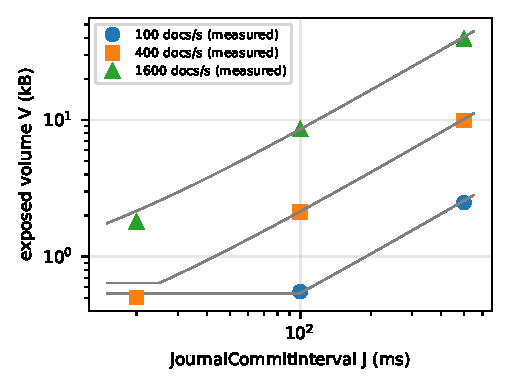
\includegraphics[width=\columnwidth]{figures/fig_plant.pdf}
\caption{Static plant: measured exposed volume versus $J$ at three loads, with the model (grey).}\label{fig:plant}
\end{figure}
\begin{table}[t]\centering\small
\caption{Static plant: measured exposed volume $V$ (kB per sync) versus the model $V=R(J+pL_0)/p$, $p=\min(1,RJ/b_0)$, $b_0=513$\,B, $L_0=7$\,ms.}\label{tab:plant}
\resizebox{\columnwidth}{!}{\begin{tabular}{rrrrrr}\toprule
Load (docs/s) & $J$ (ms) & $R$ (kB/s) & $V$ meas. & $V$ model & err. (\%)\\\midrule
100 & 500 & 5.1 & 2.49 & 2.57 & +3.4\\
100 & 100 & 5.1 & 0.56 & 0.54 & -2.3\\
100 & 20 & 5.0 & 0.50 & 0.54 & +6.9\\
400 & 500 & 20.0 & 9.92 & 10.16 & +2.4\\
400 & 100 & 20.0 & 2.13 & 2.14 & +0.7\\
400 & 20 & 20.0 & 0.50 & 0.64 & +27.8\\
1600 & 500 & 80.1 & 39.24 & 40.60 & +3.5\\
1600 & 100 & 80.0 & 8.58 & 8.57 & -0.1\\
1600 & 20 & 80.0 & 1.79 & 2.16 & +20.9\\
\bottomrule\end{tabular}}\end{table}


\paragraph{Dynamics.}
A load step from 400 to 1600 documents/s with $J$ fixed multiplied $V$ by 4.05 (at $J=100$\,ms) and 4.00
($J=200$\,ms) for a load ratio of 3.98. The 10\,s window makes the sensor the dominant dynamics: $V$ reaches 63\,\%
of its final value after 6.5--7\,s and 95\,\% after 10\,s, as expected for a moving average, whereas the
byte rate $R$ estimated tick by tick reaches 90\,\% after 2\,s. The actuator (\texttt{setParameter} plus read-back)
takes $4.9$\,ms on average (maximum 6.4\,ms), far below the 0.5\,s control period.

\paragraph{Measurement noise.}
The window average is noisy mainly because of counting: at $J=500$\,ms a 10\,s window contains about 20 syncs and one sync more or less changes $V$ by 5\,\%. The relative standard deviation of $V$
is \vcvMinFiveHundred--\vcvMaxFiveHundred\,\% at $J=500$\,ms, \vcvMinHundred--\vcvMaxHundred\,\% at 100\,ms and \vcvMinTwenty--\vcvMaxTwenty\,\% at 20\,ms (Table~\ref{tab:noise}). The per-tick
byte rate, used as load estimate, has a relative standard deviation of \rcvBaseMin--\rcvBaseMax\,\% at 400 documents/s and \rcvBurstMin--\rcvBurstMax\,\% at 1600, with a lag-one autocorrelation of
\racfBaseMin\ to \racfBaseMax\ (base) and \racfBurstMin\ to \racfBurstMax\ (burst): close to white, slightly negative because of tick-boundary counting. The noise is therefore a quantisation effect, not a drifting error,
and the steady-state error floor of 1.2--1.5\,\% seen in closed loop is of the same order.
\begin{table}[t]\centering\small
\caption{Measurement noise of the 10\,s signal $V$ (relative standard deviation over a 60\,s segment, open loop) and syncs per window.}\label{tab:noise}
\begin{tabular}{rrrr}\toprule
Load (docs/s) & $J$ (ms) & $\mathrm{sd}(V)/V$ (\%) & syncs per 10\,s\\\midrule
100 & 500 & 5.4 & 20\\
100 & 100 & 4.1 & 91\\
100 & 20 & 0.6 & 101\\
400 & 500 & 5.8 & 20\\
400 & 100 & 1.1 & 94\\
400 & 20 & 0.3 & 399\\
1600 & 500 & 5.8 & 20\\
1600 & 100 & 1.3 & 93\\
1600 & 20 & 0.4 & 448\\
\bottomrule\end{tabular}\end{table}


\section{Controllers and tuning}\label{sec:controllers}
All controllers work on $e=\ln V^*-\ln\hat V$ and command $J\in[20,500]$\,ms every 0.5\,s (Fig.~\ref{fig:scheme}).
\begin{figure}[t]\centering
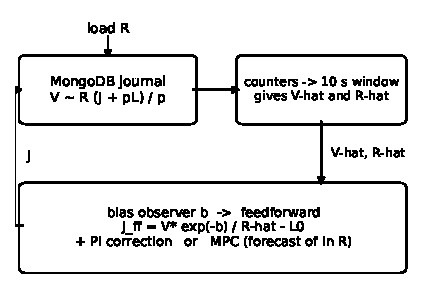
\includegraphics[width=\columnwidth]{figures/fig_scheme.pdf}
\caption{Control structure shared by all controllers. FF+obs has no PI/MPC block; PI has no feedforward; the MPC replaces the PI correction by an optimisation over a forecast of the load.}\label{fig:scheme}
\end{figure}
\paragraph{PI.} $u=\ln J=u_0+K_p e+K_i\sigma$ with integrator $\sigma\leftarrow\sigma+\Delta t\,e$ ($\Delta t=0.5$\,s), clamp or back-calculation anti-windup, and optional filtering of $\ln\hat V$. The PI acts on the windowed signal $\hat V$ (Section~\ref{sec:plant}); the load-aware controllers also use the per-tick byte rate $\hat R$.
\paragraph{Feedforward with observer (FF+obs).}
With $\hat R$ the smoothed per-tick byte rate, $J_\mathrm{ff}=V^*e^{-b}/\hat R-L_0$, where the bias
$b$ is an exponential average of $\ln V_{\rm measured}-\ln V_{\rm model}$ computed over the same 10\,s window; it
absorbs model error (floor, $p$, $L_0$) and compensates the sensor window. There is no feedback gain and no prediction.
\paragraph{PI with feedforward (PI-FF).} The same feedforward plus the PI correction; the tuner selected no bias observer for this family ($\text{bias}\_\alpha=0$) and unsmoothed load input.
\paragraph{PI on a fast estimate (PI-fast).} Added in amendment 4 to separate the value of the fast signal from that of the controller structure. The PI acts on $e=\ln V^*-\ln\hat V_{\rm fast}$ with $\ln\hat V_{\rm fast}=\ln v(\hat R,J_{k-1})+b$: the static law $v$ evaluated at the current load estimate and the last applied interval, corrected by the same bias observer as FF+obs. It has no feedforward term and no prediction. Like the other families it received 60 random candidates on the simulator, with the same seeds and the same robust objective; the retained specification is $K_p=2.75$, $K_i=0.98$, back-calculation anti-windup, filter factor 0.25, observer factor 0.6 and load smoothing 0.6, and no parameter sits on an edge of the search range. The specifications of the other families were not changed.
\paragraph{Operator baselines (amendment 6).} \emph{Static} keeps the engine default $J=100$\,ms. \emph{Threshold} is a rule-based manager of the kind found in operator scripts: on the windowed $V$, if $V/V^*>h$ it multiplies $J$ by $d<1$, if $V/V^*<l$ it multiplies $J$ by $u>1$, otherwise it holds, with at most one action every $c$ ticks and $J$ bounded. It was tuned per cell with the same budget as the other families (60 candidates); the retained specifications are $h=1.44$, $l=0.93$, $d=0.18$, $u=1.41$, $c=16$ ticks on the step, and $h=1.18$, $l=0.82$, $d=0.57$, $u=1.17$, $c=4$ ticks on the periodic load.
\paragraph{MPC.} At each tick, $u=\ln J$ minimises $\sum_{i=1}^{H}\gamma^{i-1}s(e_i)e_i^2+\lambda(u-u_{\rm prev})^2$ with
$e_i=\ln V^*-[\ln v(\hat R_{k+i},e^{u})+b]$, $v$ the static law and $s=w$ when $V$ is below the target and 1 otherwise. $\hat R_{k+i}$ is
forecast by persistence (exponentially smoothed level), moving average (level plus least-squares slope) or ARIMA(1,1,0) fitted by least squares on the
window (5 samples for the moving average and ARIMA, Table~\ref{tab:params}: these are light forecasters). The scalar problem is solved by grid search and golden-section refinement: with an additive linear model the cost is convex and a line search suffices, but with the static law $v$ convexity is not guaranteed, hence the continuous refinement of a dense grid. With a flat forecast, $H$ and $\gamma$ only rescale the move penalty: with $G=\sum_{i=1}^{H}\gamma^{i-1}$, $G e^2+\lambda\Delta^2 \equiv e^2+(\lambda/G)\Delta^2$ (up to the asymmetric weight $w$). Without move penalty ($\lambda\to0$) and with $H=1$ the MPC reduces to FF+obs (checked numerically); with $\lambda>0$ it acts as FF+obs followed by smoothing of the command, which is consistent with its smaller $|\Delta\ln J|$ (Table~\ref{tab:main}).

\paragraph{Tuning protocol.}
Each family (PI, PI-FF, FF+obs, each MPC predictor, and later PI-fast, amendment 4, and the amendment 5 and 6 families, re-tuned for each new cell) received the same budget of 60 random candidates, evaluated on a
calibrated simulator with a robust objective (half nominal plant, half stress plant with slower sync, more jitter and one tick of actuator delay),
on tuning seeds disjoint from test seeds. The three MPC predictors share the same candidates. Search ranges were widened after a first run placed continuous optima on an edge; the edge values that remain are the ``no filtering'' options (value 1) and extremes of discrete sets, listed with the tuned specifications in the repository. A first tuning gave the MPC an apparent advantage over PI-FF, traced to a different smoothing of the load estimate;
all controllers now receive the same raw inputs and tune their own smoothing. A PI with default gains is kept as a naive reference only. Table~\ref{tab:params} lists every parameter used.
\begin{table*}[t]\centering\small
\caption{Controller parameters used in all runs (random search, 60 candidates per family, robust objective; nominal values from the repository file \texttt{tuned\_specs.json}). PI-default is the naive reference (no tuning). Dashes: parameter not used by the family.}\label{tab:params}
\resizebox{\textwidth}{!}{\begin{tabular}{lccccccccccc}\toprule
Controller & $K_p$ & $K_i$ & anti-windup & $\alpha_V$ & feedforward & $\alpha_{R}$ & bias $\alpha_b$ & $H$ & $\gamma$ & $\lambda$ & $w$ (below target)\\\midrule
PI-default & 0.3 & 0.05 & clamp & 1 & no & -- & -- & -- & -- & -- & --\\
PI (tuned) & 3.19 & 0.35 & backcalc & 1 & no & -- & -- & -- & -- & -- & --\\
PI-FF & 3.66 & 0.19 & backcalc & 1 & yes & 1 & 0 & -- & -- & -- & --\\
PI-fast & 2.75 & 0.98 & backcalc & 0.25 & no (fast $\hat V$) & 0.6 & 0.6 & -- & -- & -- & --\\
FF+obs & 0.00 & 0.00 & clamp & 1 & yes & 1 & 1 & -- & -- & -- & --\\
MPC persistence & -- & -- & -- & -- & -- & 1 & 1 & 10 & 0.85 & 0.020 & 0.62\\
MPC moving average & -- & -- & -- & -- & -- & 0.3 & 1 & 3 & 0.7 & 0.024 & 0.86\\
MPC ARIMA(1,1,0) & -- & -- & -- & -- & -- & 0.3 & 1 & 3 & 0.7 & 0.024 & 0.86\\
\bottomrule\end{tabular}}
\\[2pt]{\footnotesize Common: $V^*=4096$\,B, period 0.5\,s, $J\in[20,500]$\,ms, $J_0=100$\,ms, window 10\,s, $b_0=513$\,B, $L_0=7$\,ms; MA/ARIMA window 5 / 5 samples (persistence ignores it). $\alpha_V$: filter on $\ln V$; $\alpha_R$: smoothing of the load estimate; $\alpha_b$: bias observer.}\end{table*}


\section{Experimental protocol}\label{sec:protocol}
\paragraph{Platform and workload.}
A Kind cluster (Kubernetes v1.27.3, one control plane and three workers) on a single Windows host under WSL2 (6\,GB), MongoDB 8.0.32 in a single
authenticated pod, other database workloads stopped. The generator inserts batches of 10 documents with four threads at a regulated rate,
write concern $w=1$, $j=\text{false}$ (writes are acknowledged before the journal is synchronised, so the exposure window is set by $J$). Target $V^*=4096$\,B.
\paragraph{Scenarios.} Stationary (400 documents/s); burst (400$\to$1600 documents/s from $t=100$ to 160\,s); low load (100 documents/s with the same burst, to 400 documents/s from $t=100$ to 160\,s; at 100 documents/s $V^*$ is
unreachable because $J$ would exceed 500\,ms, so the actuator saturates outside the burst). Runs last 300\,s with a 20\,s warm-up. Amendment 5 adds a triangular ramp ($400\to1600\to400$ documents/s, 60\,s up and 60\,s down from $t=100$\,s), a periodic load (raised cosine between 400 and 1600 documents/s, period 40\,s, three periods from $t=100$\,s) and a 1\,s actuation delay, injected by the runner: the command computed at tick $k$ is applied two ticks later and the controller is not told, as for an operator acting through an API.
\paragraph{Design.} Controllers are run in randomised blocks (interleaved in time), 30\,s apart. A run is invalid and repeated if a pod restarts,
the acknowledged rate falls below 95\,\% of the offered rate, or insertions fail. A pilot of 63 runs (3 per cell) preceded a campaign of 71 runs; the pilot
used the same specifications and is pooled. Cell sizes were set after the pilot from its variability (amendment recorded before the campaign) and are therefore unequal (Table~\ref{tab:main}). Pooling the pilot with the campaign, and the pod recreation between them, leave open a batch effect; none is detected on the burst error or the peak (pilot against campaign, same specifications, exact Mann--Whitney $p>0.1$ for every controller, with only 3 pilot runs per cell and hence low power); the gap between the PI and the load-aware controllers, however, is far larger than the between-run spread and is reproduced on a second platform (Section~\ref{sec:replication}).
\paragraph{Amendment 4: PI-fast block.} The amendment was written and committed to the repository before any run of this block. One block of the burst scenario compares PI-fast with the PI and FF+obs: 10 valid runs per controller, each repetition containing the three controllers in random order, 30\,s apart, with the same validity rules. It is analysed alone, with contemporaneous controls and without pooling with earlier runs. Criteria, Mann--Whitney tests with Holm correction (over the four declared contrasts: PI-fast against PI and against FF+obs, on two criteria), bootstrap CIs, Cliff's $\delta$ and TOST margins are those of the main study. Three readings were fixed in advance: (a) PI-fast equivalent to FF+obs, so the gap is due to signal speed; (b) PI-fast between the two, so signal speed explains part of the gap; (c) PI-fast equivalent to the PI, so structure matters. All 30 runs were valid.
\paragraph{Amendment 5: other disturbances and delay.} Written and committed before any run of the block. Three cells (ramp; periodic; periodic with 1\,s delay) $\times$ four controllers (PI, FF+obs, MPC with persistence, MPC with ARIMA) $\times$ 8 valid runs, in one randomised interleaved plan (96 runs). Each family was re-tuned for each cell with the equal budget. Declared contrasts per cell: FF+obs against each MPC, and the two MPC predictors against each other, with Holm correction over 18 tests; three readings were fixed in advance: (a) no predictor beats FF+obs, (b) a predictor beats it on the periodic load, (c) a predictor beats it only with delay. All 96 runs were valid.
\paragraph{Amendment 6: confirmation and baselines.} Written and committed before any run of the block (72 runs in one interleaved plan). Block A repeats the one suggestive contrast of amendment 5 (MPC with ARIMA against FF+obs on the periodic load, no delay) on 12 new valid runs per controller, with a single declared test (two-sided Mann--Whitney, $\alpha=0.05$, no correction; confirmed if $p<0.05$ and ARIMA is lower) analysed on the new runs alone. Block B compares Static and Threshold with a contemporaneous FF+obs on the step burst and the periodic load, 8 runs each, with Holm correction over 8 tests.
\paragraph{Pre-specified analysis.}
Errors are $|V/V^*-1|$ with $V$ over the 10\,s window. Primary criteria on the burst scenario: the mean error from the start of the burst to 20\,s after its end (the time the sensor window needs to forget it), called burst error below, and the exposure peak (maximum of $V$ computed over 4\,s windows, relative to $V^*$). The steady-state error is computed from $t=50$\,s. The recovery time is the time from the start of the burst until the error stays below 15\,\% for 20\,s.
Seven contrasts, Mann--Whitney tests with Holm correction over 14 tests, Cliff's $\delta$ and bootstrap CIs; equivalence (TOST on Welch 90\,\% CI)
for the pairs where the claim is ``no difference'', with margins of 0.7 percentage points (burst error) and 0.10 (peak). Margins are about
half the steady-state noise floor.

\paragraph{Use of AI assistance.}
An AI assistant (Claude, Anthropic) was used to support protocol design, to write and test the code of the controllers, the simulator, the run orchestration and the analysis scripts, to generate figures and tables, and to draft the text. All experiments were run by the authors on their own infrastructure, and all reported data come from those runs; every number in the tables and in the text is produced by the released scripts from the released run files. The authors reviewed and verified all outputs and take full responsibility for the content. The tool is not an author.

\section{Results}\label{sec:results}
\paragraph{Data.}
135 main runs (pilot 63, campaign 71, and one run added to restore $n=15$ for FF+obs after the stalled run was set aside), all valid, plus 81 sensitivity runs, 30 runs of the PI-fast block (Section~\ref{sec:pifast}), 96 runs of amendment 5 (Section~\ref{sec:scn}) and 72 runs of amendment 6 (Section~\ref{sec:amend6}), all valid; no pod restarted during any run, acknowledged/offered rate between 0.964 and 1.002. The pod was recreated once between the pilot and the campaign and restarted once between two sessions of the sensitivity campaign (13 runs before, 68 after; the concurrent nominal controls were run after).
\paragraph{Primary criteria.}
Table~\ref{tab:main} and Fig.~\ref{fig:burst}--\ref{fig:primary} summarise the burst scenario. Cell sizes are unequal ($n=\NMaePITS$ for PI, $n=\NMaePIFFS$ for PI-FF, FF+obs and MPC with persistence, $n=\NMaeMPCMS$ for MPC with a moving average; Section~\ref{sec:protocol}). The tuned PI has a burst error of \MaePITS\,\%\ (sd \MaeSdPITS) and a
peak of \PeakPITS$\times V^*$, against \MaePIFFS\,\% (PI-FF), \MaeFFOS\,\% (FF+obs) and \MaeMPCPS\,\% (MPC with persistence), with peaks of \PeakPIFFS, \PeakFFOS\ and
\PeakMPCPS. The PI-versus-PI-FF difference is $+$\cDMaePITPIFFS\ pp (95\,\% CI [\cLoMaePITPIFFS, \cHiMaePITPIFFS], $p_{\rm Holm}=\,$$\cPHMaePITPIFFS$).

\begin{figure}[t]\centering
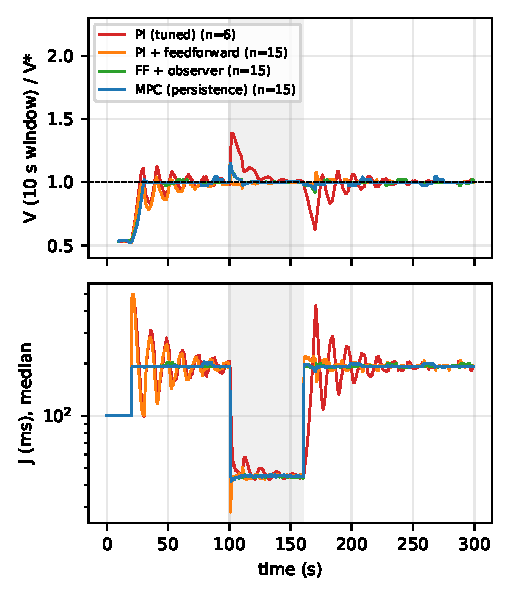
\includegraphics[width=\columnwidth]{figures/fig_burst.pdf}
\caption{Burst scenario, median over valid runs, the stalled run excluded (shaded: burst). Top: $V$ over a 10\,s window relative to the target. Bottom: commanded $J$.}\label{fig:burst}
\end{figure}
\begin{figure*}[t]\centering
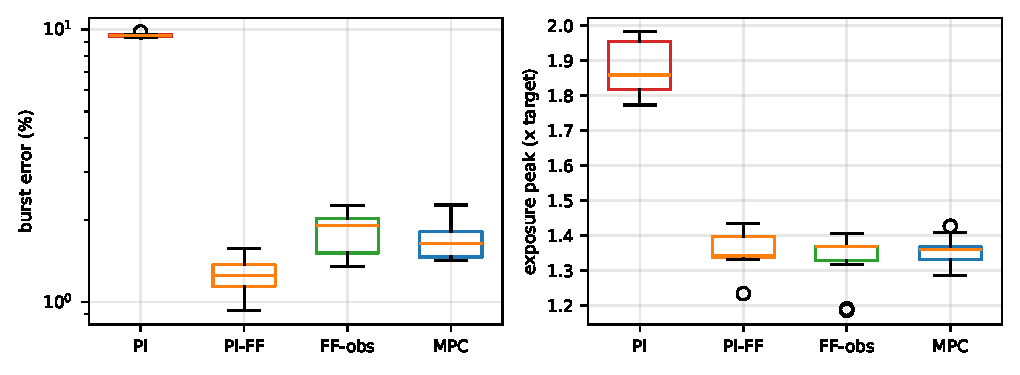
\includegraphics[width=0.8\textwidth]{figures/fig_primary.pdf}
\caption{Primary criteria per controller (boxes: quartiles; points: outliers).}\label{fig:primary}
\end{figure*}
\begin{table*}[t]\centering\small
\caption{Burst scenario (400$\to$1600 documents/s for 60 s): primary criteria and secondary measures, mean (sd) over $n$ valid runs (pilot included). The single run with a journal-sync stall $\geq 5$\,s (FF + observer) is excluded here; all contrasts are also reported with it (Table~\ref{tab:contrasts}). Peak = maximum exposure over 4\,s windows relative to the target $V^*$.}\label{tab:main}
\resizebox{0.92\textwidth}{!}{\begin{tabular}{lrcccc}\toprule
Controller & $n$ & Burst error (\%) & Peak ($\times V^*$) & Steady error (\%) & $|\Delta\ln J|$ per tick\\\midrule
PI (default gains) & 3 & 55.51 (1.80) & 2.71 (0.03) & 35.61 (0.65) & 0.005 (0.000)\\
PI (tuned) & 6 & 9.55 (0.15) & 1.88 (0.09) & 4.85 (0.13) & 0.043 (0.001)\\
PI + feedforward & 15 & 1.25 (0.17) & 1.36 (0.05) & 1.40 (0.10) & 0.055 (0.012)\\
FF + observer & 15 & 1.82 (0.30) & 1.34 (0.07) & 1.46 (0.11) & 0.032 (0.015)\\
MPC, persistence & 15 & 1.69 (0.28) & 1.36 (0.04) & 1.40 (0.12) & 0.026 (0.007)\\
MPC, moving average & 10 & 2.81 (0.45) & 1.50 (0.08) & 1.78 (0.25) & 0.024 (0.005)\\
MPC, ARIMA(1,1,0) & 10 & 1.83 (0.46) & 1.40 (0.14) & 1.59 (0.15) & 0.028 (0.009)\\
\bottomrule\end{tabular}}\end{table*}

\begin{table*}[t]\centering\small
\caption{Pre-specified contrasts (Mann--Whitney U, two-sided; Holm correction over the 14 tests = 7 contrasts $\times$ 2 primary criteria). Difference = mean(A) $-$ mean(B) with 95\% bootstrap CI; $\delta$ = Cliff's delta. ``All runs'' includes the stalled run; ``excl.'' removes it (post hoc sensitivity analysis).}\label{tab:contrasts}
\resizebox{\textwidth}{!}{\begin{tabular}{llccccc}\toprule
 & Contrast (A vs B) & Difference [95\% CI] (all runs) & $\delta$ & $p_{\text{Holm}}$ (all) & Difference [CI] (excl.) & $p_{\text{Holm}}$ (excl.)\\\midrule
\multicolumn{7}{l}{\emph{Burst error (pp)}}\\
 & PI vs PI-FF & +8.30 [+8.17, +8.44] & +1.00 & $4.4\!\times\!10^{-4}$ & +8.30 [+8.17, +8.44] & $4.4\!\times\!10^{-4}$\\
 & PI-FF vs FF+obs & -11.17 [-32.44, -0.44] & -0.93 & $1.8\!\times\!10^{-4}$ & -0.57 [-0.74, -0.40] & $2.7\!\times\!10^{-4}$\\
 & FF+obs vs MPC-pers. & +10.73 [-0.02, +32.03] & +0.35 & $0.605$ & +0.13 [-0.07, +0.32] & $0.951$\\
 & PI-FF vs MPC-pers. & -0.44 [-0.61, -0.29] & -0.92 & $2.5\!\times\!10^{-4}$ & -0.44 [-0.61, -0.29] & $2.7\!\times\!10^{-4}$\\
 & MPC-pers. vs MPC-MA & -1.12 [-1.42, -0.83] & -0.95 & $9.2\!\times\!10^{-4}$ & -1.12 [-1.42, -0.83] & $9.2\!\times\!10^{-4}$\\
 & MPC-pers. vs MPC-ARIMA & -0.14 [-0.43, +0.17] & -0.15 & $1.000$ & -0.14 [-0.43, +0.17] & $1.000$\\
 & PI vs MPC-pers. & +7.86 [+7.68, +8.03] & +1.00 & $4.4\!\times\!10^{-4}$ & +7.86 [+7.68, +8.03] & $4.4\!\times\!10^{-4}$\\
\multicolumn{7}{l}{\emph{Peak ($\times V^*$)}}\\
 & PI vs PI-FF & +0.52 [+0.45, +0.59] & +1.00 & $0.005$ & +0.52 [+0.45, +0.59] & $0.005$\\
 & PI-FF vs FF+obs & -2.33 [-7.07, +0.05] & +0.10 & $1.000$ & +0.02 [-0.01, +0.06] & $1.000$\\
 & FF+obs vs MPC-pers. & +2.34 [-0.05, +7.07] & +0.06 & $1.000$ & -0.02 [-0.06, +0.01] & $1.000$\\
 & PI-FF vs MPC-pers. & +0.00 [-0.03, +0.03] & +0.09 & $1.000$ & +0.00 [-0.03, +0.03] & $1.000$\\
 & MPC-pers. vs MPC-MA & -0.15 [-0.20, -0.09] & -0.81 & $0.005$ & -0.15 [-0.20, -0.09] & $0.005$\\
 & MPC-pers. vs MPC-ARIMA & -0.04 [-0.13, +0.04] & -0.25 & $1.000$ & -0.04 [-0.13, +0.04] & $1.000$\\
 & PI vs MPC-pers. & +0.52 [+0.46, +0.59] & +1.00 & $0.005$ & +0.52 [+0.46, +0.59] & $0.005$\\
\bottomrule\end{tabular}}\end{table*}


\paragraph{MPC versus feedforward with observer.}
FF+obs versus MPC with persistence: $+$\cDMaeFFOMPCPS\ pp [\cLoMaeFFOMPCPS, \cHiMaeFFOMPCPS] on the burst error ($p_{\rm Holm}=\,$$\cPHMaeFFOMPCPS$) and
\cDPeakFFOMPCPS\ on the peak. The equivalence tests (Table~\ref{tab:equiv}) conclude to equivalence on both criteria once the stalled run (below) is set aside, and are
inconclusive with it (one extreme value widens the CI), while the rank tests do not change.
MPC with a moving average has a burst error larger than persistence by \cAMaeMPCPMPCMS\ pp, and ARIMA is equivalent to persistence on the burst error;
neither forecaster improves on persistence.
\begin{table}[t]\centering\small
\caption{Equivalence tests (TOST, Welch 90\% CI inside $\pm$ margin; margins 0.7\,pp on the burst error and 0.10 on the peak).}\label{tab:equiv}
\resizebox{\columnwidth}{!}{\begin{tabular}{lccc}\toprule
Pair, criterion & 90\% CI (excl.) & verdict (excl.) & verdict (all)\\\midrule
FF+obs vs MPC-pers., error & [-0.05, +0.31] & equivalent & inconclusive\\
MPC-pers. vs MPC-ARIMA, error & [-0.42, +0.15] & equivalent & equivalent\\
FF+obs vs MPC-pers., peak & [-0.05, +0.01] & equivalent & inconclusive\\
MPC-pers. vs MPC-ARIMA, peak & [-0.12, +0.04] & inconclusive & inconclusive\\
\bottomrule\end{tabular}}\end{table}


\paragraph{PI with feedforward.}
On the main platform PI-FF has the lowest burst error, \cAMaePIFFMPCPS\ pp below MPC (Table~\ref{tab:contrasts}), with no difference on the exposure peak; this did not replicate on the second platform (Section~\ref{sec:replication}). It also moves $J$ about twice as much
(\ChatPIFFS\ against \ChatMPCPS\ in $|\Delta\ln J|$ per tick) and, when the target is unreachable and the actuator saturates (low-load scenario), recovers in \LowRecPIFFS\,s against \LowRecMPCPS\,s
for MPC (Table~\ref{tab:other}; descriptive, $n=6$).
\begin{table}[t]\centering\small
\caption{Stationary (400 documents/s) and low-load (100$\to$400 documents/s, target unreachable at the start) scenarios, mean over $n_{\rm st}$ stationary runs and $n_{\rm ll}$ low-load runs (stationary runs: pilot only, descriptive).}\label{tab:other}
\resizebox{\columnwidth}{!}{\begin{tabular}{lccccc}\toprule
Controller & Stat. err. (\%) & Low-load err. (\%) & Recov. (s) & $n_{\rm st}$ & $n_{\rm ll}$\\\midrule
PI-def. & 26.08 & 49.83 & -- & 3 & 3\\
PI & 1.32 & 28.78 & 1.8 & 3 & 6\\
PI-FF & 1.38 & 31.48 & 24.1 & 3 & 6\\
FF+obs & 1.34 & 28.18 & 2.9 & 3 & 6\\
MPC-pers. & 1.22 & 28.01 & 3.0 & 3 & 6\\
MPC-MA & 1.31 & 28.22 & 2.3 & 3 & 6\\
MPC-ARIMA & 1.49 & 28.27 & 2.8 & 3 & 6\\
\bottomrule\end{tabular}}\end{table}


\paragraph{A journal-sync stall.}
One run (FF+obs, first run after the pod was recreated) shows no journal sync for 12.5\,s during the burst, then 1.5\,s and 1\,s; its burst error is 171\,\% and its peak $39\times V^*$. It is valid under the
pre-specified rules and is included in the primary analysis; the sensitivity analysis excludes runs with a sync gap of 5\,s or more (a rule defined from the counters, post hoc). The cause is unknown; two shorter gaps (1 and 1.5\,s) occur in two other runs of the main analysis, and one gap of 3.5\,s in a sensitivity run (the PI-FF run at $K_p\times1.5$ discussed in Section~\ref{sec:sens}). Counters of journal pre-allocation are now recorded to investigate such events.

\paragraph{Simulator versus real cluster.}
The simulator was calibrated on the static grid (worst error 3.9\,\% on $V$) and on the burst response. On the pilot the ranking of the seven controllers by burst error is identical to the simulated
one (Spearman 1.00), with real-to-simulated ratios between 0.80 and 1.09. The simulator underestimates the steady-state measurement noise (real error 1.2--1.5\,\% versus 0.5--0.95\,\%) and the between-run variability,
so it was used for tuning and design only.

\subsection{PI on a fast estimate of $V$ (amendment 4)}\label{sec:pifast}
The block of Section~\ref{sec:protocol} separates signal speed from controller structure. Table~\ref{tab:pifast} gives the result. PI-fast has a burst error of 5.01\,\% (sd 0.75), between the PI (9.62\,\%) and FF+obs (1.93\,\%) measured in the same block; these two controls agree with the main study (9.55\,\% and 1.82\,\%, Table~\ref{tab:main}). The four declared contrasts are significant after Holm correction ($p_{\rm Holm}=0.0007$ each, Cliff's $\delta=\pm1$). PI-fast minus PI is $-4.61$ pp on the burst error (95\,\% CI [$-5.00$, $-4.09$]) and $-0.25$ on the peak ([$-0.29$, $-0.20$]); PI-fast minus FF+obs is $+3.09$ pp ([2.62, 3.62]) and $+0.21$ ([0.18, 0.24]). No equivalence was concluded. The distributions do not overlap: the worst PI-fast run (6.90\,\%) is below the best PI run (9.33\,\%) and above the worst FF+obs run (2.97\,\%). PI-fast closes 60\,\% of the burst-error gap between PI and FF+obs (95\,\% CI 53--66\,\%) and 55\,\% of the peak gap (44--67\,\%): the second pre-specified reading. No run of the block had a journal-sync gap above 1.0\,s.
\begin{table}[t]\centering\small
\caption{PI-fast block (amendment 4), burst scenario, mean (sd) over 10 valid runs per controller run contemporaneously and analysed alone. Last row: share of the PI-to-FF+obs difference closed by PI-fast, with 95\,\% bootstrap CI.}\label{tab:pifast}
\begin{tabular}{lccc}\toprule
Controller & Burst error (\%) & Peak ($\times V^*$) & Recovery (s)\\\midrule
PI (tuned) & 9.62 (0.22) & 1.87 (0.07) & 11.00 (0.00)\\
PI-fast & 5.01 (0.75) & 1.62 (0.04) & 8.75 (0.86)\\
FF + observer & 1.93 (0.43) & 1.41 (0.04) & 2.00 (0.41)\\\midrule
Gap closed by PI-fast & 60\,\% [53, 66] & 55\,\% [44, 67] & --\\
\bottomrule\end{tabular}\end{table}

One observation was not expected. The burst error of PI-fast increases with the order of the runs (Spearman $\rho=0.82$, $p=0.004$; 4.45--4.70\,\% in the first five runs, 4.75--6.90\,\% in the last five), whereas no significant trend appears for the PI ($\rho=0.55$, $p=0.10$) or FF+obs ($\rho=0.15$, $p=0.68$). We did not investigate the cause; since PI-fast depends on the static model through $\hat V_{\rm fast}$, a slow change of the plant is a possible but untested explanation. The ordering of the three controllers does not depend on it, but the PI-fast mean should be read as the average of a drifting quantity.

\subsection{Other disturbances and actuation delay (amendment 5)}\label{sec:scn}
Table~\ref{tab:scn} gives the 96 runs. In none of the 18 declared tests does a predictor beat FF+obs after Holm correction. On the ramp, MPC with persistence (1.16\,\%) and FF+obs (1.49\,\%) cannot be told apart (difference 0.33 pp, 95\,\% CI [$-0.04$, 0.88], $p_{\rm H}=1$); FF+obs has a larger spread there (sd 0.73 pp) because of one slow run. On the periodic load, MPC with ARIMA has the lowest error (1.95\,\% against 2.47\,\% for FF+obs; difference 0.53 pp, CI [0.26, 0.79], unadjusted $p=0.005$, $p_{\rm H}=0.084$): suggestive, not significant under the declared correction, which is why amendment 6 repeats it; persistence is equivalent to FF+obs. With the 1\,s delay every controller degrades (FF+obs 6.25\,\%) and the PI collapses (17.2\,\%, no recovery inside the window); ARIMA is on average lower than FF+obs (5.64\,\%, $p_{\rm H}=0.17$) but with a spread six times larger (sd 1.01 against 0.16 pp) and a higher peak ($1.41$ against $1.31\times V^*$, not significant). No trend with run order appears (all Spearman $p>0.2$).
\begin{table}[t]\centering\small
\caption{Amendment 5: other disturbances and actuation delay, mean (sd) over 8 valid runs per cell and controller. Error = mean $|V/V^*-1|$ over the disturbance window (\%); peak in $\times V^*$. Each family was re-tuned for each cell. $p_{\rm H}$: Mann--Whitney $p$ of the controller against FF+obs after Holm correction over the 18 declared tests.}\label{tab:scn}
\begin{tabular}{llcccc}\toprule
Cell & Controller & Error (\%) & Peak & $p_{\rm H}$ (error) & Recovery (s)\\\midrule
Ramp & PI & 4.93 (0.21) & 1.20 (0.10) & -- & 1.0\\
 & FF+obs & 1.49 (0.73) & 1.13 (0.15) & -- & 4.3\\
 & MPC persistence & 1.16 (0.10) & 1.07 (0.02) & 1 & 1.0\\
 & MPC ARIMA & 1.20 (0.23) & 1.08 (0.02) & 1 & 1.0\\\midrule
Periodic & PI & 10.06 (0.11) & 1.30 (0.04) & -- & 46.3\\
 & FF+obs & 2.47 (0.36) & 1.15 (0.04) & -- & 1.0\\
 & MPC persistence & 2.21 (0.22) & 1.13 (0.03) & 1 & 1.0\\
 & MPC ARIMA & 1.95 (0.18) & 1.12 (0.04) & 0.084 & 1.0\\\midrule
Periodic, 1\,s delay & PI & 17.17 (0.17) & 1.67 (0.05) & -- & 125.6\\
 & FF+obs & 6.25 (0.16) & 1.31 (0.03) & -- & 1.0\\
 & MPC persistence & 6.48 (1.05) & 1.35 (0.17) & 1 & 7.2\\
 & MPC ARIMA & 5.64 (1.01) & 1.41 (0.27) & 0.17 & 7.0\\
\bottomrule\end{tabular}\end{table}

\subsection{Confirmation and operator baselines (amendment 6)}\label{sec:amend6}
Table~\ref{tab:amend6} gives the 72 runs. The declared test of block A is confirmed on the new runs: on the periodic load MPC with ARIMA has a burst error of 1.85\,\% (sd 0.28) against 2.26\,\% (0.15) for FF+obs, a difference of $-0.40$ pp (95\,\% CI [$-0.56$, $-0.21$], Cliff's $\delta=-0.83$, $p=0.0006$); the peak is unchanged ($-0.001\times V^*$) and the I/O cost is the same (8.65 against 8.63 synchronisations per second). The gain is about 18\,\% of the error. In block B the baselines are far from the load-aware controller: the static default has a burst error of 89.4\,\% on the step and 50.9\,\% on the periodic load, with an exposure peak of $2.2\times V^*$; the threshold rules reduce it to 18.3\,\% and 24.1\,\% (peak 2.16 and $2.05\times V^*$) and some runs do not recover inside the run, against 1.76\,\% and 2.52\,\% for FF+obs. All eight declared contrasts are significant after Holm correction ($p_{\rm H}\le0.0036$, Cliff's $\delta=1$). None of the baselines saves synchronisation work: 9.4 syncs/s for the static default and 8.5 and 10.0 for the threshold rules, against 8.6 for FF+obs.
\begin{table}[t]\centering\small
\caption{Amendment 6. Top: confirmation block on the periodic load (12 new valid runs per controller, runs 9 to 20), mean (sd). Bottom: operator baselines against a contemporaneous FF+obs, 8 valid runs per cell and controller. Static: $J=100$\,ms never changed; Threshold: rule-based manager. Error in \%, peak in $\times V^*$, I/O cost in journal synchronisations per second. All eight contrasts against FF+obs are significant after Holm correction ($p_{\rm H}\le 0.0036$).}\label{tab:amend6}
\begin{tabular}{llcccc}\toprule
Block & Controller & Error (\%) & Peak & Syncs/s & Cliff $\delta$ vs FF+obs\\\midrule
Confirmation, periodic & FF+obs & 2.26 (0.15) & 1.13 (0.02) & 8.63 & --\\
 & MPC ARIMA & 1.85 (0.28) & 1.13 (0.03) & 8.65 & $-0.83$ ($p=0.0006$)\\\midrule
Baselines, step burst & Static & 89.38 (1.72) & 2.24 (0.04) & 9.39 & 1.00\\
 & Threshold & 18.28 (1.79) & 2.16 (0.05) & 8.51 & 1.00\\
 & FF+obs & 1.76 (0.30) & 1.35 (0.03) & 8.62 & --\\\midrule
Baselines, periodic & Static & 50.89 (0.80) & 2.24 (0.12) & 9.39 & 1.00\\
 & Threshold & 24.09 (1.13) & 2.05 (0.07) & 10.00 & 1.00\\
 & FF+obs & 2.52 (0.33) & 1.20 (0.12) & 8.62 & --\\
\bottomrule\end{tabular}\end{table}

\subsection{Sensitivity to parameters and to the target}\label{sec:sens}
The criteria below were fixed before the runs (amendment 2). Each continuous parameter of PI, PI-FF, FF+obs and MPC (persistence) was perturbed one at a time by $\times0.5$ and $\times1.5$ (clipped to valid values), 3 runs per variant, with 3 concurrent nominal runs per controller
(Table~\ref{tab:sens}); the target was also changed (Table~\ref{tab:vstar}). The analysis is descriptive ($n=3$): ranges and ratios, no tests.
\paragraph{C1, parameter robustness.}
Worst ratio of burst error to the concurrent nominal: PI \SensWorstPIT, FF+obs \SensWorstFFO, MPC \SensWorstMPCP, PI-FF \SensWorstPIFF\ (driven by one run, see below; about 1.7 without it). For FF+obs and MPC the only large ratio comes from one parameter, the smoothing of the load estimate:
halving its factor multiplies the burst error by \SensSmoothFFO\ (FF+obs) and \SensSmoothMPCP\ (MPC), and by \SensSmoothPIFF\ for PI-FF, where halving the integral gain matters as much (2.63). The MPC weights ($\lambda$, $w$) and the observer factor change the error by $-10$ to $+16$\,\%.
PI-FF is the only controller with an unstable run: with $K_p\times1.5$ ($K_p=5.5$), one of three runs oscillated (burst error 10.5\,\%, peak $20\times V^*$) while the other two did not (1.8 and 2.0\,\%, peak $1.18\times V^*$); the means of Table~\ref{tab:sens} (\SensPIFFkpErr\,\%, \SensPIFFkpPeak$\times V^*$) are driven by that run. It coincides with a journal-sync stall of 3.5\,s, so with $n=3$ we cannot separate an effect of the gain from an effect of the stall.
\paragraph{C2, robustness of the ranking.}
On the burst error the worst load-aware variant (\SensWorstAwareErr\,\%) is below the best PI variant (\SensBestPIErr\,\%): the ranking survives. On the exposure peak it survives for FF+obs (largest peak \SensMaxPeakFFO) and for MPC (\SensMaxPeakMPCP)
against the best PI variant (\SensMinPeakPIT) but not for PI-FF (\SensPIFFkpPeak, a mean driven by the single run above). As specified, over the union of the three load-aware families, C2 is therefore \emph{not} satisfied on the peak; we report it as such.
\paragraph{C3, target.}
Journal syncs per second follow $1/V^*$ (about 17, 8.6 and 4.3 per second for $V^*=2048$, 4096 and 8192\,B, Table~\ref{tab:vstar}), the cost of a tighter target. No controller is uniformly best across targets;
at the unreachable $V^*=2048$\,B the MPC has a larger error than FF+obs.
\begin{table}[t]\centering\small
\caption{Sensitivity to controller parameters (burst scenario, $n=3$ per variant, one-at-a-time, descriptive). Ratios are relative to 3 concurrent nominal runs of the same controller. Nominal: PI \MaeSensPITnom\,\%, PI-FF \MaeSensPIFFnom\,\%, FF+obs \MaeSensFFOnom\,\%, MPC \MaeSensMPCPnom\,\%.}\label{tab:sens}
\resizebox{\columnwidth}{!}{\begin{tabular}{llcccc}\toprule
Controller & Variant & Error (\%) & Ratio & Peak ($\times V^*$) & $|\Delta\ln J|$\\\midrule
PI & $K_i\times0.5$ & 14.79 & 1.58 & 1.82 & 0.041\\
PI & $K_i\times1.5$ & 8.07 & 0.86 & 2.08 & 0.048\\
PI & $K_p\times0.5$ & 11.35 & 1.21 & 2.16 & 0.024\\
PI & $K_p\times1.5$ & 8.52 & 0.91 & 1.77 & 0.063\\
PI-FF & $\alpha_R\times0.5$ & 2.44 & 2.16 & 1.47 & 0.048\\
PI-FF & $K_i\times0.5$ & 2.98 & 2.63 & 1.32 & 0.057\\
PI-FF & $K_i\times1.5$ & 1.33 & 1.18 & 1.42 & 0.059\\
PI-FF & $K_p\times0.5$ & 1.47 & 1.30 & 1.33 & 0.043\\
PI-FF & $K_p\times1.5$ & 4.76 & 4.20 & 7.45 & 0.094\\
FF+obs & $\alpha_b\times0.5$ & 1.68 & 1.02 & 1.41 & 0.029\\
FF+obs & $\alpha_R\times0.5$ & 3.18 & 1.93 & 1.54 & 0.016\\
MPC-pers. & $\alpha_b\times0.5$ & 1.43 & 0.90 & 1.36 & 0.020\\
MPC-pers. & $\alpha_R\times0.5$ & 3.70 & 2.32 & 1.61 & 0.023\\
MPC-pers. & $\lambda\times0.5$ & 1.85 & 1.16 & 1.37 & 0.032\\
MPC-pers. & $\lambda\times1.5$ & 1.49 & 0.93 & 1.33 & 0.023\\
MPC-pers. & $w\times0.5$ & 1.51 & 0.95 & 1.33 & 0.026\\
MPC-pers. & $w\times1.5$ & 1.47 & 0.92 & 1.42 & 0.023\\
\bottomrule\end{tabular}}\end{table}

\begin{table}[t]\centering\small
\caption{Change of the target $V^*$ (burst, $n=3$): error, peak and journal syncs per second. At $V^*=2048$\,B the target is unreachable during the burst ($J$ would be below 20\,ms).}\label{tab:vstar}
\begin{tabular}{llccc}\toprule
Controller & $V^*$ (B) & Error (\%) & Peak & syncs/s\\\midrule
PI-FF & 2048 & 2.33 & 1.34 & 17.02\\
PI-FF & 4096 & 1.13 & 1.40 & 8.68\\
PI-FF & 8192 & 2.32 & 1.47 & 4.41\\
FF+obs & 2048 & 1.74 & 1.32 & 17.23\\
FF+obs & 4096 & 1.64 & 1.39 & 8.62\\
FF+obs & 8192 & 2.83 & 1.40 & 4.31\\
MPC-pers. & 2048 & 4.90 & 1.57 & 16.76\\
MPC-pers. & 4096 & 1.60 & 1.37 & 8.61\\
MPC-pers. & 8192 & 3.68 & 1.39 & 4.28\\
\bottomrule\end{tabular}\end{table}


\subsection{Replication on a second platform}\label{sec:replication}
To reduce the single-host limitation, the burst scenario was replayed for four controllers (PI, PI-FF, FF+obs, MPC with persistence), 6 runs each, on a shared GitHub-hosted Linux runner
(\CICpu, 4 vCPU, \CIRam\,GB, kernel \CIKernel) with MongoDB \CIImage\ in plain Docker, without WSL2 or Kubernetes. The specifications were not re-tuned. MongoDB 8.x refuses to start on this kernel
(SERVER-121912, an allocator incompatibility); the community workaround \texttt{GLIBC\_TUNABLES=glibc.pthread.rseq=1} was applied. It concerns the memory allocator, not the journal path, but its effect on the
measurements is not verified. Three criteria were fixed before the runs: R1 (the PI burst error is at least three times that of each load-aware controller), R2 (FF+obs and MPC equivalent, same margins as above) and R3
(the PI exposure peak is the highest). All \CIN\ runs were valid.
Table~\ref{tab:ci} gives the results. R1 is \CIRone\ (ratios \CIRatioPIFF, \CIRatioFFO\ and \CIRatioMPCP), R2 is \CIRtwo\ (error difference \CIeqMaeD\ pp, 90\,\% CI [\CIeqMaeLo, \CIeqMaeHi]; peak difference
\CIeqPeakD, [\CIeqPeakLo, \CIeqPeakHi]) and R3 is \CIRthree. One finding did not replicate: on the main platform PI-FF had a lower burst error than MPC ($-$\cAMaePIFFMPCPS\ pp); on the second platform the difference is
\CIPIFFvsMPCD\ pp (95\,\% CI [\CIPIFFvsMPCLo, \CIPIFFvsMPCHi]), so the sign of the difference is the opposite of the main platform: it is platform-dependent and should not be generalised.
The second platform widens the range of hosts, not the topology: it is still a single node.
\begin{table}[t]\centering\small
\caption{Replication on a second platform (shared Linux runner, MongoDB in plain Docker), burst scenario, mean (sd) over 6 runs; last column: same controller on the main platform.}\label{tab:ci}
\resizebox{\columnwidth}{!}{\begin{tabular}{lccccc}\toprule
Controller & Error (\%) & Peak ($\times V^*$) & $|\Delta\ln J|$ & syncs/s & Main platform (\%)\\\midrule
PI (tuned) & 9.36 (0.27) & 1.86 (0.11) & 0.044 & 8.54 & 9.55\\
PI + feedforward & 1.52 (0.06) & 1.38 (0.06) & 0.046 & 8.70 & 1.25\\
FF + observer & 1.45 (0.32) & 1.37 (0.03) & 0.022 & 8.63 & 1.82\\
MPC, persistence & 1.33 (0.12) & 1.37 (0.03) & 0.019 & 8.63 & 1.69\\
\bottomrule\end{tabular}}\end{table}


\section{Discussion}\label{sec:discussion}
\paragraph{Why prediction does not help here.}
The actuator acts on $V$ within one control tick, while the sensor is delayed by the 10\,s window. A controller that knows $\hat R$ and the static law can therefore set $J$ almost
exactly; what remains is to correct the sensor lag and model error, which the bias observer does. Forecasting $R$ several ticks ahead adds noise, not information, because the plant has no
delay to compensate: with a moving average the burst error is worse, although this variant was also tuned with a smoother load estimate ($\alpha_R=0.3$ against 1 for persistence, Table~\ref{tab:params}), which alone roughly doubles the burst error of the persistence MPC when halved (Table~\ref{tab:sens}); the effect of the slope term is therefore not isolated. This is consistent with the equivalence of MPC and FF+obs. A step burst cannot be anticipated by any forecaster, so we also tested a ramp, a periodic load and a 1\,s actuation delay (Sections~\ref{sec:scn} and~\ref{sec:amend6}). Forecasting helps a little on the periodic load: ARIMA lowers the burst error by 0.4 pp (about 18\,\%), confirmed on 12 new runs per controller. A periodic load of fixed period is the case a forecaster is built for, and the gain is small; persistence forecasting does not help, the ramp shows no gain, and with a 1\,s delay the gain is not significant while the spread of the MPC is six times larger. The conclusion that forecasting is not needed therefore holds for steps and ramps, and becomes a conclusion of small gain for a deterministic periodic load.
\paragraph{Why feedback alone fails.}
Feedback on the windowed $V$ reacts only as the window fills. Even with a high proportional gain ($K_p=3.2$, $K_i=0.35$ after tuning) the PI shows a
burst error five to eight times larger than PI-FF, FF+obs and MPC with persistence, and a peak 1.4 times higher (Fig.~\ref{fig:burst}); in the 50--100\,s that precede the burst its error fluctuates more around the target than that of the other controllers (standard deviation of $V/V^*$ about 3.7\,\% against 2.0--2.9\,\%). The main comparison does not separate feedforward from fast measurement; amendment 4 does: a PI acting on a fast model-based estimate of $V$ (computed from $\hat R$, the last applied interval and the static law) recovers about 60\,\% of the gap to FF+obs (Section~\ref{sec:pifast}). Most of the benefit of the load-aware designs therefore comes from the speed of the signal, and the remaining 40\,\% from acting on the load directly rather than through an error; a plausible reason, which we did not test, is that a feedback loop must still see an error before it reacts, even on a fast estimate. A Smith predictor and a PI on a purely measured short-window $V$ were not tested.
\paragraph{Against operator practice.}
The comparison that matters most to an operator is not MPC against feedforward. The engine default leaves the exposure at $2.2\times V^*$ during a burst (89\,\% burst error on the step, 51\,\% on the periodic load) and threshold rules, even tuned, keep it at 18--24\,\% error, against under 3\,\% for a load feedforward with an observer, at the same or lower I/O cost. Having any load-aware control in the loop is worth roughly an order of magnitude in exposure error here; which load-aware design is used is a second-order choice.
\paragraph{What matters.}
The controller structure matters less than the responsiveness of the load estimate: smoothing it more than the plant requires doubles the burst error for every load-aware controller (Table~\ref{tab:sens}), while the MPC weights and the observer factor are second order (for PI-FF, the integral gain matters as much).
\paragraph{Practical guidance.}
On this engine and knob, a load feedforward with a model-bias observer is the simplest controller that attains the accuracy of MPC and it was stable over the two perturbations tested (the others are clipped by the parameter bounds, Table~\ref{tab:sens}). On the main platform PI with feedforward has the lowest nominal burst error (not replicated on the second platform) and the only unstable run of the sensitivity analysis (one of three runs at a 50\,\% higher gain, coinciding with a journal-sync stall);
it also moves the actuator twice as much and recovers more slowly under saturation. We therefore see feedback as optional: useful only with a gain margin that is measured, not assumed. With a 1\,s actuation delay the feedforward degrades gracefully (6.3\,\% error, sd 0.16 pp) where the PI collapses (17.2\,\%).

\section{Limitations}\label{sec:limits}
(i) One engine and single-node deployments on two hosts (Kind under WSL2, and a shared Linux runner with MongoDB in Docker for the burst scenario only, which required a community workaround for a kernel incompatibility of MongoDB 8.x whose effect on the measurements is not verified); (ii) $V$ is a composite of two counters and no crash-recovery experiment verifies it as data loss;
(iii) the simulator underestimates noise and between-run variability; (iv) tuning was done on the simulator and checked on a pilot; (v) one run contains a long journal-sync stall of unknown cause;
(vi) in the sensitivity analysis one of three PI-FF runs at a 50\,\% higher gain oscillated, coinciding with a journal-sync stall of 3.5\,s, so the instability cannot be attributed to the gain; the simulator does not oscillate at that gain unless one extra tick of delay is added, so unmodelled delay is a plausible but unverified cause; (vii) the pod restarted once between two sessions of the sensitivity campaign (each run individually valid); (viii) equivalence margins are set from the noise floor and a different margin could change an ``inconclusive'' into ``equivalent'' or the reverse; (ix) the sensitivity analysis is descriptive ($n=3$ per variant) and one-at-a-time, so interactions between parameters are not explored;
(x) one profile of each disturbance (step, ramp, periodic load of period 40\,s) and one actuation delay (1\,s): other periods, amplitudes and delays are untested, and the ARIMA gain was measured on a deterministic periodic profile, the most favourable case for a forecaster;
(xi) PI-fast uses the same static model as FF+obs to estimate $V$, was tested in a block of 10 runs per controller, and its burst error drifts with the run order for an unidentified reason; a PI on a purely measured short-window $V$ and a Smith predictor were not tested;
(xii) the moving-average and ARIMA forecasters are light (5-sample window, ARIMA(1,1,0)) and were tuned with a smoother load estimate than persistence ($\alpha_R=0.3$ against 1), so the comparison does not isolate the forecaster; richer forecasters were not explored;
(xiii) cell sizes are unequal, the pilot is pooled with the campaign and the pod was recreated between them;
(xiv) $V$ is an exposure proxy in bytes for a single node; no replication-level RPO is measured;
(xv) the baselines do not cover all operator practice (no proprietary autoscaler, no manual tuning by an administrator); the threshold cooldown (16 ticks on the step) and, for MPC with persistence, the horizon (20 ticks, the longest of the set, on the ramp and periodic cells) sit at the edge of the search sets and longer values were not tried;
(xvi) with 8 runs per cell the contrasts of amendment 5 that are not significant after correction should not be read as no effect; only the periodic ARIMA contrast was confirmed on new runs.

\section{Conclusion}\label{sec:conclusion}
On a real MongoDB deployment, using the observed write load is what lets a controller hold the exposed journal volume near its target during bursts; a PI fed with a fast model-based estimate of that volume already recovers about 60\,\% of the gap to a feedforward, so most of the gain is signal speed. Under a step burst, a model predictive controller with persistence forecasting is equivalent to a plain
feedforward with a model-bias observer (once one stalled run is set aside), and forecasting the load with a moving average or ARIMA does not help. In the descriptive sensitivity analysis the advantage of the feedforward does not depend on a precise tuning, except for the responsiveness of the load estimate, and a feedback term should be added only with a measured gain margin (one of three PI-FF runs oscillated at a 50\,\% higher gain). The ordering of PI against the load-aware controllers and the equivalence of MPC and feedforward with observer replicated on a second platform; the lower burst error of PI with feedforward did not. Forecasting helps only slightly and only on a periodic load, where ARIMA lowers the error by about 0.4 pp (18\,\%), confirmed on new runs; on a ramp and with a 1\,s actuation delay no gain was shown. Against operator practice the gain of any load-aware control is large: the engine default and tuned threshold rules have 18--89\,\% burst error against under 3\,\% for a feedforward. These conclusions are limited to the engine, the disturbance profiles and the platforms tested.

\section*{Declarations}
\textbf{Funding.} No funding was received. \textbf{Competing interests.} The authors declare no competing interests.
\textbf{Ethics approval.} Not applicable: the study involves no human participants or animals.
\textbf{Author contributions.} All authors contributed to the study conception and design. The experiments, data collection and analysis were performed by I.~Jerrari. All authors read and approved the final manuscript.
\textbf{Data availability.} The run files of the main study, of the sensitivity analysis and of the replication, the run schedules, the tuned specifications and the amendments written before each data collection are available at
\url{https://github.com/imanejerrari-etu-bit/mpc-rpo-mongodb}, release \texttt{v1.0}\repoRef.
\textbf{Code availability.} The code (\texttt{mpcrpo}), the analysis scripts and the sources of this manuscript are in the same repository and release.


\begin{thebibliography}{9}
\bibitem{camacho2013model}
E.\ F.\ Camacho and C.\ Bordons.
\newblock \emph{Model Predictive Control}.
\newblock Advanced Textbooks in Control and Signal Processing.
  Springer-Verlag London, 2nd edition, 2007.

\bibitem{muske2002disturbance}
K.\ R.\ Muske and T.\ A.\ Badgwell.
\newblock Disturbance modeling for offset-free linear model predictive
  control.
\newblock \emph{Journal of Process Control}, 12(5):617--632, 2002.

\bibitem{pannocchia2003disturbance}
G.\ Pannocchia and J.\ B.\ Rawlings.
\newblock Disturbance models for offset-free model-predictive control.
\newblock \emph{AIChE Journal}, 49(2):426--437, 2003.

\bibitem{kothare1994antiwindup}
M.\ V.\ Kothare, P.\ J.\ Campo, M.\ Morari, and C.\ N.\ Nett.
\newblock A unified framework for the study of anti-windup designs.
\newblock \emph{Automatica}, 30(12):1869--1883, 1994.

\bibitem{astrom1989windup}
K.\ J.\ {\AA}str\"om and L.\ Rundqwist.
\newblock Integrator windup and how to avoid it.
\newblock In \emph{Proceedings of the 1989 American Control
  Conference}, pp.\ 1693--1698. IEEE, 1989.

\bibitem{roy2011autoscaling}
N.\ Roy, A.\ Dubey, and A.\ Gokhale.
\newblock Efficient autoscaling in the cloud using predictive models
  for workload forecasting.
\newblock In \emph{Proceedings of the IEEE 4th International
  Conference on Cloud Computing (CLOUD'11)}, pp.\ 500--507, 2011.

\bibitem{gong2010press}
Z.\ Gong, X.\ Gu, and J.\ Wilkes.
\newblock PRESS: PRedictive Elastic ReSource Scaling for cloud
  systems.
\newblock In \emph{Proceedings of the International Conference on
  Network and Service Management (CNSM)}, pp.\ 9--16, 2010.

\bibitem{cai2022inverse}
Z.\ Cai and R.\ Buyya.
\newblock Inverse queuing model-based feedback control for elastic
  container provisioning of web systems in Kubernetes.
\newblock \emph{IEEE Transactions on Computers}, 71(2):337--348, 2022.

\bibitem{pozdniakova2024sla}
O.\ Pozdniakova, D.\ Ma\v{z}eika, and A.\ Cholomskis.
\newblock SLA-adaptive threshold adjustment for a Kubernetes
  horizontal pod autoscaler.
\newblock \emph{Electronics}, 13(7):1242, 2024.

\bibitem{serracanta2025stability}
B.\ Serracanta, A.\ Luk\'acs, A.\ Rodriguez-Natal, A.\ Cabellos, and
  G.\ R\'etv\'ari.
\newblock On the stability of the Kubernetes horizontal autoscaler
  control loop.
\newblock \emph{IEEE Access}, 13:7160--7166, 2025.

\bibitem{baresi2016discrete}
L.\ Baresi, S.\ Guinea, A.\ Leva, and G.\ Quattrocchi.
\newblock A discrete-time feedback controller for containerized cloud
  applications.
\newblock In \emph{Proceedings of the 24th ACM SIGSOFT International
  Symposium on Foundations of Software Engineering (FSE 2016)}, pp.\
  217--228, 2016.

\bibitem{sabuhi2021adaptive}
M.\ Sabuhi, N.\ Mahmoudi, and H.\ Khazaei.
\newblock Optimizing the performance of containerized cloud software
  systems using adaptive PID controllers.
\newblock \emph{ACM Transactions on Autonomous and Adaptive Systems},
  15(3), 2021.

\bibitem{vanaken2017ottertune}
D.\ Van Aken, A.\ Pavlo, G.\ J.\ Gordon, and B.\ Zhang.
\newblock Automatic database management system tuning through
  large-scale machine learning.
\newblock In \emph{Proceedings of the 2017 ACM International
  Conference on Management of Data (SIGMOD'17)}, pp.\ 1009--1024, 2017.

\bibitem{zhang2019cdbtune}
J.\ Zhang, Y.\ Liu, K.\ Zhou, G.\ Li, Z.\ Xiao, B.\ Cheng, J.\ Xing,
  Y.\ Wang, T.\ Cheng, L.\ Liu, M.\ Ran, and Z.\ Li.
\newblock An end-to-end automatic cloud database tuning system using
  deep reinforcement learning.
\newblock In \emph{Proceedings of the 2019 ACM International
  Conference on Management of Data (SIGMOD'19)}, pp.\ 415--432, 2019.

\bibitem{ferreira2020selftunable}
L.\ Ferreira, F.\ Coelho, and J.\ Pereira.
\newblock Self-tunable DBMS replication with reinforcement learning.
\newblock In \emph{Distributed Applications and Interoperable Systems
  (DAIS 2020)}, LNCS vol.\ 12135, pp.\ 131--147. Springer, 2020.

\bibitem{joshi2024arimapid}
N.\ S.\ Joshi, R.\ Raghuwanshi, Y.\ M.\ Agarwal, B.\ Annappa, and
  D.\ N.\ Sachin.
\newblock ARIMA-PID: container auto scaling based on predictive
  analysis and control theory.
\newblock \emph{Multimedia Tools and Applications}, 83(9):26369--26386,
  2024.

\bibitem{kusic2009lookahead}
D.\ Kusic, J.\ O.\ Kephart, J.\ E.\ Hanson, N.\ Kandasamy, and G.\ Jiang.
\newblock Power and performance management of virtualized computing
  environments via lookahead control.
\newblock \emph{Cluster Computing}, 12(1):1--15, 2009.

\bibitem{padala2009automated}
P.\ Padala, K.-Y.\ Hou, K.\ G.\ Shin, X.\ Zhu, M.\ Uysal, Z.\ Wang,
  S.\ Singhal, and A.\ Merchant.
\newblock Automated control of multiple virtualized resources.
\newblock In \emph{Proceedings of the 4th ACM European Conference on
  Computer Systems (EuroSys'09)}, pp.\ 13--26, 2009.

\bibitem{fang2016qos}
Q.\ Fang, J.\ Wang, and Q.\ Gong.
\newblock QoS-driven power management of data centers via model
  predictive control.
\newblock \emph{IEEE Transactions on Automation Science and
  Engineering}, 13(4):1557--1566, 2016.

\bibitem{astrom2008feedback}
K.\ J.\ {\AA}str\"om and R.\ M.\ Murray.
\newblock \emph{Feedback Systems: An Introduction for Scientists and
  Engineers}.
\newblock Princeton University Press, 2008.
\end{thebibliography}
\end{document}
